\documentclass[10pt]{book}

\usepackage[letterpaper,top=2.5cm,bottom=2.5cm,left=2.5cm,right=2.5cm]{geometry}
\usepackage[T1]{fontenc}
\usepackage[utf8]{inputenc}
\usepackage{graphicx}
\usepackage{multicol}
\usepackage{multirow}
\usepackage[normalem]{ulem}
\usepackage{float}
\usepackage{amsmath}
\usepackage{amsthm}
\usepackage{amsfonts}
\usepackage[usenames,dvipsnames,table]{xcolor}
\usepackage{xspace}
\usepackage{xhfill}
\usepackage{fancyhdr}
\usepackage[nolist]{acronym}
\usepackage{listings}
% note sure after here
\usepackage{makeidx}
\usepackage[UKenglish]{isodate}
\usepackage{ifthen}
\usepackage{textcomp}
\usepackage{alltt}
\usepackage{ifpdf}
\ifpdf
\usepackage[pdftex,
            pagebackref=true,
            colorlinks=true,
            linkcolor=blue,
            unicode
           ]{hyperref}
\else
\usepackage[ps2pdf,
            pagebackref=true,
            colorlinks=true,
            linkcolor=blue,
            unicode
           ]{hyperref}
\usepackage{pspicture}
\fi
\usepackage{sectsty}
\usepackage{mathptmx}
\usepackage[scaled=.90]{helvet}
\usepackage{courier}
\usepackage[titles]{tocloft}
\usepackage{prettyref}
\usepackage{mdwlist}
\usepackage{enumitem}
\usepackage{framed}
\usepackage{pbox}
\usepackage{draftcopy}
\usepackage{draftwatermark}
\usepackage{wrapfig}
\usepackage{longtable}
\usepackage{caption}
\usepackage{subcaption}
\usepackage{csquotes}


\definecolor{ListingBG}{rgb}{0.91,0.91,0.91}
\definecolor{shadecolor}{rgb}{0.92,0.92,0.92}

\hyphenation{Open-SHMEM}

\renewcommand{\chaptername}{Chapter} 
\renewcommand{\appendixname}{Annex} 

% Place some penalty for doing the break
% The penalty for a ``\gb'' should be greater than a \hyphenpenalty.
% \hyphenpenalty is 50 in plain.tex.
\def\gb{\penalty10000\hskip 0pt plus 8em\penalty4800\hskip 0pt plus-8em%
\penalty10000}

% This macro enables that all "_" (underscore) characters in the pfd
% file are searchable, and that cut&paste will copy the "_" as underscore. 
% Without the following macro, the \_ is treated in searches and cut&paste
% as a " " (space character). 
% This macro does not modify the behavior of _ in math or in verbatim 
% environments. In verbatim environments, the "_" is always treated
% as a searchable character.
%
\DeclareRobustCommand{\_}{\texttt{\char`\_}} 
% 

\def\colorswapnt{\colorlet{saved}{.}\color{ForestGreen}}
\def\colorswapot{\colorlet{saved}{.}\color{red}}
\def\prevcolor{\color{saved}}

\newcommand{\newtext}[1]{\textcolor{ForestGreen}{#1}}
\newcommand{\oldtext}[1]{\textcolor{magenta}{\sout{#1}}}
\newcommand{\insertDocVersion}{1.4}
\newcommand{\openshmem}[1][]{%
  {Open\-SHMEM\ifthenelse{\equal{#1}{}}{}{~#1}}\xspace}
\newcommand{\HEADER}[1]{\textit{#1}}
\newcommand{\FUNC}[1]{\textit{#1}}
\newcommand{\CTYPE}[1]{\textit{#1}}
\newcommand{\VAR}[1]{\textit{#1}}
\newcommand{\CONST}[1]{\textit{#1}}
\newcommand{\const}[1]{\protect\gb\protect{\textsf{\small #1}}\index{CONST:#1}} % Only library_constants.tex table.
\newcommand{\CorCpp}{\textit{C/C++}\xspace}
\newcommand{\CorCppFor}{\textit{C/C++/Fortran}\xspace}
\newcommand{\Fortran}[1][]{%
  \textit{Fortran\ifthenelse{\equal{#1}{}}{}{~#1}}\xspace}
\newcommand{\Cstd}[1][]{%
  \textit{C\ifthenelse{\equal{#1}{}}{}{#1}}\xspace}
\newcommand{\Cpp}[1][]{%
  \textit{C++\ifthenelse{\equal{#1}{}}{}{#1}}\xspace}
\newcommand{\TYPE}{\emph{TYPE}}
\newcommand{\TYPENAME}{\emph{TYPENAME}}
\newcommand{\SIZE}{\emph{SIZE}}

\newcommand{\source}{\textit{source}}
\newcommand{\dest}{\textit{dest}}
\newcommand{\PUT}{\textit{Put}}
\newcommand{\GET}{\textit{Get}}
\newcommand{\OPR}[1]{\textit{#1}}
\newcommand{\barrier}{\FUNC{SHMEM\_BARRIER}\xspace} % why here an not others?
\newcommand{\barrierall}{\FUNC{SHMEM\_BARRIER\_ALL}\xspace} % why here an not others?
\newcommand{\broadcast}{\FUNC{SHMEM\_BROADCAST}}
\newcommand{\collect}{\FUNC{SHMEM\_COLLECT}}
\newcommand{\fcollect}{\FUNC{SHMEM\_FCOLLECT}}
\newcommand{\reduction}{\textit{Reduction Operations}}
\newcommand{\alltoall}{\FUNC{SHMEM\_ALLTOALL}}
\newcommand{\alltoalls}{\FUNC{SHMEM\_ALLTOALLS}}
\newcommand{\activeset}{\textit{Active~set}\xspace} % why here and not others?
\newcommand{\shmemprefix}{\textit{SHMEM\_}}
\newcommand{\shmemprefixLC}{\textit{shmem\_}}
\newcommand{\shmemprefixC}{\textit{\_SHMEM\_}}
\newcommand{\ith}{${\textit{i}^{\text{\tiny th}}}$}
\newcommand{\jth}{${\textit{j}^{\text{\tiny th}}}$}
\newcommand{\kth}{${\textit{k}^{\text{\tiny th}}}$}
\newcommand{\lth}{${\textit{l}^{\text{\tiny th}}}$}

\begin{acronym}
\acro{RMA}{\emph{Remote Memory Access}}
\acro{RMO}{\emph{Remote Memory Operation}}
\acro{AMO}{\emph{Atomic Memory Operation}}
\acro{PE}{\emph{Processing Element}}
\acrodefplural{PE}[PEs]{\emph{Processing Elements}}
\acro{PGAS}{\emph{Partitioned Global Address Space}}
\acro{API}{\emph{Application Programming Interface}}
\acro{MPI}{\emph{Message Passing Interface}}
\acro{SPMD}{\emph{Single Program Multiple Data}}
\acro{ARL}{Army Research Laboratory}
\acro{AMD}{Advanced Micro Devices}
\acro{UH}{University of Houston}
\acro{UO}{University of Oregon}
\acro{ORNL}{Oak Ridge National Laboratory}
\acro{LANL}{Los Alamos National Laboratory}
\acro{ESSC}{Extreme Scale Systems Center}
\acro{OSSS}{Open Software System Solutions}
\acro{DoD}{U.S. Department of Defense}
\acro{SBU}{Stonybrook University}
\acro{UTK}{University of Tenneesee at Knoxville}
\end{acronym}


%
% This is used to put line numbers on plain pages.  Used in draft.tex
%
\makeatletter

\def\withlinenumbers{\relax
  \def\@evenfoot{\hbox to 0pt{\hss\LineNumberRuler\hskip 1.5pc}\hfil}\relax
  \def\@oddfoot{\hfil\hbox to 0pt{\hskip 1.5pc\LineNumberRuler\hss}}}

\def\LineNumberRuler{\vbox to 0pt{\vss\normalsize \baselineskip13.6pt
    \lineskip 1pt \normallineskip 1pt \def\baselinestretch{1}\relax
    \LNR{1}\LNR{2}\LNR{3}\LNR{4}\LNR{5}\LNR{6}\LNR{7}\LNR{8}\LNR{9}
    \LNR{10}\LNR{11}\LNR{12}\LNR{13}\LNR{14}
        \LNR{15}\LNR{16}\LNR{17}\LNR{18}\LNR{19}
    \LNR{20}\LNR{21}\LNR{22}\LNR{23}\LNR{24}
        \LNR{25}\LNR{26}\LNR{27}\LNR{28}\LNR{29}
    \LNR{30}\LNR{31}\LNR{32}\LNR{33}\LNR{34}\LNR{35}
        \LNR{36}\LNR{37}\LNR{38}\LNR{39}
    \LNR{40}\LNR{41}\LNR{42}\LNR{43}\LNR{44}
        \LNR{45}\LNR{46}\LNR{47}\LNR{48}
    \vskip 31pt}}
\def\LNR#1{\hbox to 1pc{\hfil\tiny#1\hfil}}

\def\ps@plainwithlinenumbers{\let\@mkboth\@gobbletwo
     \def\@oddhead{}
     \def\@oddfoot{\hfil\rm\thepage\hfil
       \hbox to 0pt{\hskip 1.5pc\LineNumberRuler\hss}}
     \def\@evenhead{}
     \def\@evenfoot{\hbox to 0pt{\hss
     \LineNumberRuler\hskip 1.5pc}\rm\hfil\thepage\hfil}}

    % Contents is done with \chapter*{Contents}, so we need to turn off the
    % line numbers in this case.  Easiest to look at def

\newwrite\chappages
\immediate\openout\chappages=chappage.txt
\def\writespace{ }

\def\incontents{0}
\newif\ifcontents
\contentsfalse
\def\chapter{\clearpage \ifcontents\else\thispagestyle{plainwithlinenumbers}\fi
        \write\chappages{Chapter \thechapter\writespace - \the\count0}
        \global\@topnum\z@ \@afterindentfalse \secdef\@chapter\@schapter}

\makeatother

%
% End this is used to put line numbers on plain pages.  Used in draft.tex
%

%
% Use Sans Serif font for sections, etc.
%
\makeatletter
\def\section{\@startsection {section}{1}{\z@}{-3.5ex plus -1ex minus 
-.2ex}{2.3ex plus .2ex}{\Large\sf}}
\def\subsection{\@startsection{subsection}{2}{\z@}{-3.25ex plus -1ex minus 
-.2ex}{1.5ex plus .2ex}{\large\sf}}
\def\subsubsection{\@startsection{subsubsection}{3}{\z@}{-3.25ex plus 
-1ex minus -.2ex}{1.5ex plus .2ex}{\normalsize\sf\bf}}
\def\paragraph{\@startsection {paragraph}{4}{\z@}{3.25ex plus 1ex 
minus .2ex}{-1em}{\normalsize\sf}}
\makeatother
%
% End use Sans Serif font for sections, etc.  S. Otto
%


%
% This section is for example code listings
%
\definecolor{gray}{rgb}{0.92,0.92,0.92}

\lstset{ % set defaults for languages not otherwise defined
  breakatwhitespace=false,         % sets if automatic breaks should only happen at whitespace
  basicstyle=\ttfamily\footnotesize,
  breaklines=true,                 % sets automatic line breaking
  escapeinside={|}{|},          % if you want to add LaTeX within your code
  extendedchars=true,              % lets you use non-ASCII characters; for 8-bits 
                                   % encodings only, does not work with UTF-8
  keepspaces=true,                 % keeps spaces in text, useful for keeping indentation of code 
                                   % (possibly needs columns=flexible)
  morekeywords={*,...},            % if you want to add more keywords to the set
  showspaces=false,                % show spaces everywhere adding particular underscores; 
                                   % it overrides 'showstringspaces'
  showstringspaces=false,          % underline spaces within strings only
  showtabs=false,                  % show tabs within strings adding particular underscores
}

\def\StandardListing {
  \lstset {
    breakatwhitespace=false,         % sets if automatic breaks should only happen at whitespace
    basicstyle=\ttfamily\footnotesize,
    breaklines=true,                 % sets automatic line breaking
    escapeinside={\%*}{*)},          % if you want to add LaTeX within your code
    extendedchars=true,              % lets you use non-ASCII characters; for 8-bits 
                                     % encodings only, does not work with UTF-8
    keepspaces=true,                 % keeps spaces in text, useful for keeping
                                     % indentation of code (possibly needs columns=flexible)
    morekeywords={*,...},            % if you want to add more keywords to the set
    showspaces=false,                % show spaces everywhere adding particular underscores; 
                                     % it overrides 'showstringspaces'
    showstringspaces=false,          % underline spaces within strings only
    showtabs=false,                  % show tabs within strings adding particular underscores
    backgroundcolor=\color{gray}, 
  }
}

\def\ProgramNumberedListing {
  \StandardListing
  \lstset {
    numbers=left,
    numberstyle=\footnotesize
  }
}

\newcommand{\numberedlisting}[2] {
  \ProgramNumberedListing
  \lstinputlisting[#1]{#2}
  \StandardListing
}

\newcommand{\outputlisting}[2] {
\begin{minipage}{\linewidth}
\vspace{0.1in}
  \lstinputlisting[#1]{#2}
  \StandardListing
\vspace{0.1in}
\end{minipage}
}

\lstdefinelanguage{OSH+C}[]{C}{
  classoffset=1,
  morekeywords={
    SHMEM_BCAST_SYNC_SIZE, SHMEM_SYNC_VALUE,
    start_pes,
    my_pe, _my_pe, shmem_my_pe,
    num_pes, _num_pes, shmem_n_pes,
    shmem_int_p, shmem_short_p, shmem_long_p,
    shmem_int_put, shmem_short_put, shmem_long_put,
    shmem_barrier_all, shmem_barrier,
    shmalloc,  shfree, shrealloc,
    shmem_broadcast32, shmem_broadcast64,
    shmem_short_inc, shmem_int_inc, shmem_long_inc,
    shmem_short_add, shmem_int_add, shmem_long_add,
    shmem_short_finc, shmem_int_finc, shmem_long_finc,
    shmem_short_fadd, shmem_int_fadd, shmem_long_fadd,
    shmem_set_lock, shmem_test_lock, shmem_clear_lock,
    shmem_long_sum_to_all,
    shmem_complexd_sum_to_all,
  },
  keywordstyle=\color{black}\textbf,
  classoffset=0,
  sensitive=true
}

\lstdefinelanguage{OSH2+C}[]{OSH+C}{
  classoffset=1,
  morekeywords={
    shmem_init,
    shmem_finalize,
    shmem_malloc,
    shmem_my_pe,
    shmem_error,
    shmem_global_exit,
  },
  keywordstyle=\color{black}\textbf,
  classoffset=0,
  sensitive=true
}

\lstdefinelanguage{OSH+F}[]{Fortran}{
  classoffset=1,
  morekeywords={
    SHMEM_BCAST_SYNC_SIZE, SHMEM_SYNC_VALUE,
    start_pes,
    my_pe, shmem_my_pe,
    num_pes, shmem_n_pes,
    shmem_int_p, shmem_short_p, shmem_long_p,
    shmem_int_put, shmem_short_put, shmem_long_put,
    shmem_barrier_all, shmem_barrier,
    shpalloc,  shpdeallc, shpclmove,
    shmem_broadcast32, shmem_broadcast64,
    shmem_broadcast4, shmem_broadcast8,
    shmem_short_inc, shmem_int_inc, shmem_long_inc,
    shmem_short_add, shmem_int_add, shmem_long_add,
    shmem_short_finc, shmem_int_finc, shmem_long_finc,
    shmem_short_fadd, shmem_int_fadd, shmem_long_fadd,
    shmem_set_lock, shmem_test_lock, shmem_clear_lock,
    shmem_long_sum_to_all,
  },
  keywordstyle=\color{black}\textbf,
  classoffset=0,
  sensitive=false
}

\lstdefinelanguage{OSH2+F}[]{OSH+F}{
  classoffset=1,
  morekeywords={
    shmem_init,
    shmem_finalize,
    shmem_malloc,
    shmem_my_pe,
    shmem_error,
    shmem_global_exit,
  },
  keywordstyle=\color{black}\textbf,
  classoffset=0,
  sensitive=true
}

%
% End this section is for example code listings
%

%
% Deprecation Helpers
%

\newcommand{\strikeline}[1][red]{{\color{#1}\raisebox{.5ex}{\rule{1em}{.4pt}}}}
\newcommand{\stretchline}[1][red]{\xrfill[.5ex]{.4pt}[#1]}
\newcommand{\DeprecationStart}[1][red]{{\color{#1} deprecation start} \mbox{}}
\newcommand{\DeprecationEnd}[1][red]{{\color{#1} deprecation end} \mbox{}}

\newcommand{\StartDeprecateBlock}{
  {\strikeline\mbox{} \DeprecationStart \stretchline\mbox{}}}
\newcommand{\EndDeprecateBlock}{%
  \mbox{}\stretchline\mbox{} \DeprecationEnd \strikeline}

\newenvironment{DeprecateBlock}{%
  \par \StartDeprecateBlock \par}{\par \EndDeprecateBlock \par}

\newcommand{\StartInlineDeprecate}{%
  \strikeline\mbox{} \DeprecationStart \strikeline \mbox{}}
\newcommand{\EndInlineDeprecate}{%
  \strikeline\mbox{} \DeprecationEnd \strikeline}
\newenvironment{DeprecateInline}{\StartInlineDeprecate}{\EndInlineDeprecate}

%
% Library API description template commands
%

\newcommand{\apisummary}[1]{
    #1
\hfill
}

\newenvironment{apidefinition}{
\begin{description}
\item[SYNOPSIS] \hfill \\ \\ 
\vspace{-2em}
}
{
\end{description}
}

\lstnewenvironment{Cpp11synopsis}
{
  \textbf{C++11:}
  \lstset{language={C++}, backgroundcolor=\color{gray}, lineskip=2pt,
  morekeywords={size_t, TYPE, noreturn}, aboveskip=0pt, belowskip=0pt}}{}

\lstnewenvironment{C11synopsis}
{ 
  \textbf{C11:} 
  \lstset{language={C}, backgroundcolor=\color{gray}, lineskip=2pt,
  morekeywords={size_t, TYPE, _Noreturn, shmem_cmp},
  aboveskip=0pt, belowskip=0pt}}{}

\lstnewenvironment{CsynopsisCol}
{ 
  \lstset{language={C}, backgroundcolor=\color{gray}, lineskip=2pt,
  morekeywords={size_t, TYPE, TYPENAME, SIZE, shmem_cmp},
  aboveskip=0pt, belowskip=0pt}}{}


\lstnewenvironment{Csynopsis}
{ 
  \textbf{C/C++:} 
  \lstset{language={C}, backgroundcolor=\color{gray}, lineskip=2pt,
  morekeywords={size_t, TYPE, TYPENAME, SIZE, shmem_cmp},
  aboveskip=0pt, belowskip=0pt}}{}

\lstnewenvironment{CsynopsisST}
{ 
  \textbf{C/C++:} 
  \color{red}  
  {\lstset{language={C}, backgroundcolor=\color{gray}, lineskip=2pt,
  morekeywords={size_t}, aboveskip=0pt, belowskip=0pt}}
  }
  {}
  
\lstnewenvironment{Fsynopsis}
{ \textbf{FORTRAN:} 
  \lstset{language={Fortran}, backgroundcolor=\color{gray}, lineskip=3pt,
  deletekeywords=[2]{STATUS},
  deletekeywords=[3]{LOG}, aboveskip=0pt,
  belowskip=0pt}}{}

\newenvironment{apiarguments}{
\newcommand{\apiargument}[3]{
\begin{tabular}{p{2cm} p{2cm} p{10cm}}
\textbf{##1} & \textit{##2} & {##3} \\ 
\end{tabular}
}
\hfill
\item[DESCRIPTION] \hfill 

\begin{description}
\item[Arguments] \hfill \\
}
{
\hfill
\end{description}
}

\newcommand{\apidescription}[1]{
\begin{description}
\vspace{-1em}
\item[API description] \hfill \\ 
    #1
\hfill
}

\newcommand{\apidesctable}[4] {\hfill \\ #1 \\ \\
    \begin{tabular}{p{5cm} p{9cm}}
       \hline
       #2 & #3 \\
       \hline \tabularnewline
       \end{tabular}\\
        #4
}  

\newcommand{\apireturnvalues}[1]{
\hfill 
\item[Return Values] \hfill \\
    #1
\\
\hfill
}

\newcommand{\apitablerow}[2]{
 \begin{tabular}{p{5cm} p{9cm}}
 #1 & #2 \tabularnewline
  \end{tabular}\\
}

\newcommand{\apinotes}[1]{
\item[Notes] \hfill \\
    #1
\hfill \\
\end{description}
}

\newcommand{\apiimpnotes}[1]{
\begin{description}
\item[Note to implementors] \hfill \\
    #1
\hfill \\
\end{description}
}

\newenvironment{apiexamples}{
\newcommand{\apicexample}[3]{
    ##1
    \lstinputlisting[language={C}, tabsize=2,
    basicstyle=\ttfamily\footnotesize, morekeywords={size_t}]{##2}
    ##3 }
\newcommand{\apifexample}[3]{
    ##1
    \lstinputlisting[language={Fortran}, tabsize=2,
    basicstyle=\ttfamily\footnotesize, deletekeywords={TARGET}]{##2}
    ##3 }
\vspace{-2pt}
\item[EXAMPLES] \hfill \\
\vspace{-2pt}
}
{
}

%
% End library API description template commands
%


\makeindex

\begin{document}

\hypersetup{pageanchor=true,citecolor=blue}

% Set header/footer for opening content
\pagestyle{fancy}
\fancyhead{}
\fancyhead[LE,LO]{\insertDocVersion}
\fancyhead[CO,CE]{--- DRAFT ---}
\SetWatermarkText{DRAFT}
\SetWatermarkScale{1}
\SetWatermarkLightness{.91}
\fancyfoot[CE,CO]{\thepage} %affects page numbering for the first pages, 
                            %except the first ToC page

\pagenumbering{roman} %sets coverpage and toc page numbers to roman numerals

\thispagestyle{empty}
\begin{center}
\textbf{\Huge \openshmem}
\par
\end{center}

\begin{center}
\textbf{\LARGE Application Programming Interface}\\
\includegraphics[scale=0.65]{figures/OpenSHMEM_Pound}\\
\url{http://www.openshmem.org/}
\par
\end{center}

\begin{center}
Version \insertDocVersion
\par
\end{center}

\vspace{0.5in}
\begin{center}
\today
\end{center}

\vspace{0.5in}

\vfill{}

\section*{Developed by}
\begin{itemize}
\item High Performance Computing Tools group at the University of Houston\\
  \url{http://www.cs.uh.edu/~hpctools/} 
\item Extreme Scale Systems Center, Oak Ridge National Laboratory\\
  \url{http://www.csm.ornl.gov/essc/} 
\end{itemize}
\pagebreak{}

\section*{Sponsored by}
\begin{itemize}
\item \ac{DoD}\\
  \url{http://www.defense.gov/ }
\item \ac{ORNL}\\
  \url{http://www.ornl.gov/} 
\end{itemize}

\section*{Authors and Collaborators}
\begin{itemize}
\item Monika ten Bruggencate, Cray Inc.
\item David Knaak, Cray Inc.
\item Jens Manser, \ac{DoD}
\item Nick Park, \ac{DoD}
\item Lauren Smith, \ac{DoD}
\item James Dinan, Intel
\item Jeff Hammond, Intel
\item Jeff Kuehn, \ac{LANL}
\item Swaroop Pophale, Mellanox
\item Eduardo D'Azevedo, \ac{ORNL}
\item Manjunath Gorentla Venkata, \ac{ORNL}
\item Oscar Hernandez, \ac{ORNL}
\item Gregory Koenig, \ac{ORNL}
\item Graham Lopez, \ac{ORNL}
\item Pavel Shamis, \ac{ORNL}
\item Steve Poole, OSSS
\item Karl Feind, SGI
\item Michael Raymond, SGI
\item Barbara Chapman, \ac{UH} 
\item Tony Curtis, \ac{UH}
\item Sameer Shende, \ac{UO}
\end{itemize}

\date{\today}

\section*{Acknowledgements}
The \openshmem specification belongs to Open Source Software Solutions, Inc.
(OSSS), a non-profit organization, under an agreement with SGI. The development
work of the specification is supported by the Oak Ridge National Laboratory
Extreme Scale Systems Center and the Department of Defense.\\
\\
We would also like to acknowledge the contribution of the members of the
\openshmem mailing list for their ideas, discussions, suggestions, and
constructive criticism which has helped us improve this document.




\setcounter{tocdepth}{4}
\setcounter{secnumdepth}{4}
\tableofcontents

\mainmatter  % included for use of documenttype 'book' 

% Set header/footer for main content
\pagestyle{fancy}   %replacing {headings} with {fancy} for customization 
\withlinenumbers    %adds line numbers to edges of normal pages
\fancyhf{}
\fancyhead[RE, LO]{\rightmark}
\fancyhead[RO, LE]{\thepage}
\renewcommand{\headrulewidth}{0pt}
\renewcommand{\thesection}{\arabic{section}}

{ %using setlength to force standardized spacing, if needed
% this command is ended in backmatter.tex
%\setlength{\baselineskip}{3pt plus 3pt minus 3pt}

\setlength{\parskip}{3pt}





\section*{Introduction}\label{sec:intro}

\section{The \openshmem Effort}\label{subsec:openshmem_effort}
\openshmem is a \ac{PGAS} library interface specification. \openshmem aims to
provide a standard \ac{API} for SHMEM libraries to aid portability and
facilitate uniform predictable results of \openshmem programs by explicitly
stating the behavior and semantics of the \openshmem library calls. Through the
different versions, \openshmem will continue to address the requirements of the
\ac{PGAS} community.  As of this specification, many existing vendors support
\openshmem-compliant implementations and new vendors are developing
\openshmem library implementations to help the users write portable \openshmem
code. This ensures that programs can run on multiple platforms without having to
deal with subtle vendor-specific implementation differences. For more details on
the history of \openshmem please refer to the
\hyperref[sec:openshmem_history]{History of \openshmem} section.  

The \openshmem\footnote{The \openshmem specification is owned by Open Source
Software Solutions Inc., a non-profit organization, under an agreement with
SGI.}  effort is driven by the \ac{ESSC} at \ac{ORNL} and the University of
Houston with significant input from the \openshmem community. Besides the
specification, the effort also includes providing a reference \openshmem
implementation, validation and verification suites, tools, a mailing list and
website infrastructure to support specification activities. For more information
please refer to: \url{http://www.openshmem.org/}.


\section{Programming Model Overview}\label{subsec:programming_model}
\openshmem implements \ac{PGAS} by defining remotely accessible data objects as
mechanisms to share information among \openshmem processes or \acp{PE}, and
private data objects that are accessible by only the \ac{PE} itself. The \ac{API}
allows communication and synchronization operations on both private (local to
the PE initiating the operation) and remotely accessible data objects. The key
feature of \openshmem is that data transfer operations are
\textit{\textbf{one-sided}} in nature. This means that a local \ac{PE} executing
a data transfer routine does not require the participation of the remote \ac{PE}
to complete the routine. This allows for overlap between communication and
computation to hide data transfer latencies, which makes  \openshmem ideal for
unstructured, small/medium size data communication patterns. The \openshmem
library routines have the potential to provide a low-latency, high-bandwidth
communication \ac{API} for use in highly parallelized scalable programs.  

The \openshmem interfaces can be used to implement \ac{SPMD} style programs.
It provides interfaces to start the \openshmem \acp{PE} in parallel and
communication and synchronization interfaces to access remotely accessible data
objects across \acp{PE}. These interfaces can be leveraged to divide a problem
into multiple sub-problems that can be solved independently or with coordination
using the communication and synchronization interfaces.  The \openshmem
specification defines library calls, constants, variables, and language bindings
for \Cstd and \Fortran%
\footnote{As of \openshmem[1.4], the \Fortran interface has been deprecated.}.
The \Cpp interface is currently the same as that
for \Cstd. Unlike Unified Parallel C, \Fortran[2008], Titanium, X10, and Chapel, which are all
PGAS languages, \openshmem relies on the user to use the library calls  to
implement the correct semantics of its programming model.

An overview of the \openshmem routines is described below:

\begin{enumerate}

\item \textbf{Library Setup and Query}
\begin{enumerate}
  \item \OPR{Initialization}: The \openshmem library environment is initialized,
   where the \acp{PE} are either single or multithreaded. 
  \item \OPR{Query}: The local \ac{PE} may get the number of \acp{PE} running
      the same program and its unique integer identifier. 
  \item \OPR{Accessibility}: The local \ac{PE} can find out if a remote \ac{PE} is
      executing the same binary, or if a particular symmetric data object can be
      accessed by a remote \ac{PE}, or may obtain a pointer to a symmetric data
      object on the specified remote \ac{PE} on shared memory systems.
\end{enumerate}

\item \textbf{Symmetric Data Object Management}
\begin{enumerate}
  \item \OPR{Allocation}: All executing \acp{PE} must participate in the
      allocation of a symmetric data object with identical arguments.
  \item  \OPR{Deallocation}: All executing \acp{PE} must participate in the
      deallocation of the same symmetric data object with identical arguments.
  \item  \OPR{Reallocation}: All executing \acp{PE} must participate in the
      reallocation of the same symmetric data object with identical arguments.
\end{enumerate}

\item \textbf{Communication Management}
\begin{enumerate}
    \item \OPR{Contexts}: Contexts are containers for communication operations.
        Each context provides an environment where the operations performed on
        that context are ordered and completed independently of other operations
        performed by the application.
\end{enumerate}

\item \textbf{Remote Memory Access}
\begin{enumerate}
    \item \PUT: The local \ac{PE} specifies the \source{} data object (private
        or symmetric) that is copied to the symmetric data object on the remote
        \ac{PE}. 
  \item \GET: The local \ac{PE} specifies the symmetric data object on the remote
      \ac{PE} that is copied to a data object (private or symmetric) on the local
      \ac{PE}. 
\end{enumerate}

\item \textbf{Atomics}
\begin{enumerate}
    \item \OPR{Swap}: The \ac{PE} initiating the swap gets the old value of a
        symmetric data object from a remote \ac{PE} and copies a new value to
        that symmetric data object on the remote \ac{PE}.
  \item \OPR{Increment}: The \ac{PE} initiating the increment adds 1 to the
      symmetric data object on the remote \ac{PE}.
  \item \OPR{Add}: The \ac{PE} initiating the add specifies the value to be added
      to the symmetric data object on the remote \ac{PE}.
  \item \OPR{Compare and Swap}: The \ac{PE} initiating the swap gets the old value
      of the symmetric data object based on a value to be compared and copies a
      new value to the symmetric data object on the remote \ac{PE}.
  \item \OPR{Fetch and Increment}: The \ac{PE} initiating the increment adds 1 to
      the symmetric data object on the remote \ac{PE} and returns with the old
      value.
  \item \OPR{Fetch and Add}: The \ac{PE} initiating the add specifies the value to
      be added to the symmetric data object on the remote \ac{PE} and returns with
      the old value.
\end{enumerate}

\item \textbf{Synchronization and Ordering}
\begin{enumerate}
  \item \OPR{Fence}: The \ac{PE} calling fence ensures ordering of   
  \PUT, AMO, and memory store operations
  to symmetric data objects with respect to a specific
      destination \ac{PE}. 
  \item \OPR{Quiet}: The \ac{PE} calling quiet ensures remote completion of remote access
      operations and stores to symmetric data objects. 
  \item \OPR{Barrier}: All or some \acp{PE} collectively synchronize and ensure
      completion of all remote and local updates prior to any \ac{PE} returning
      from the call.
\end{enumerate}

\item \textbf{Collective Communication}
\begin{enumerate}
  \item \OPR{Broadcast}: The \textit{root} \ac{PE} specifies a symmetric data
      object to be copied to a symmetric data object on one or more remote
      \acp{PE} (not including itself). 
  \item \OPR{Collection}: All \acp{PE} participating in the routine get the result
      of concatenated symmetric objects contributed by each of the \acp{PE} in
      another symmetric data object.
  \item \OPR{Reduction}: All \acp{PE} participating in the routine get the result
      of an associative binary routine over elements of the specified symmetric
      data object on another symmetric data object. 
\end{enumerate}

\item \textbf{Mutual Exclusion}
\begin{enumerate}
  \item \OPR{Set Lock}: The \ac{PE} acquires exclusive access to the region
      bounded by the symmetric \textit{lock} variable.
  \item \OPR{Test Lock}: The \ac{PE} tests the symmetric \textit{lock} variable
      for availability.
  \item \OPR{Clear Lock}: The \ac{PE} which has previously acquired the
      \textit{lock} releases it.
\end{enumerate}

\item \textbf{Data Cache Control \textit{(deprecated)}}
\begin{enumerate}
  \item Implementation of mechanisms to exploit the capabilities of hardware cache
      if available.
\end{enumerate}
\end{enumerate}


\section{Memory Model}\label{subsec:memory_model}
\begin{figure}[h]
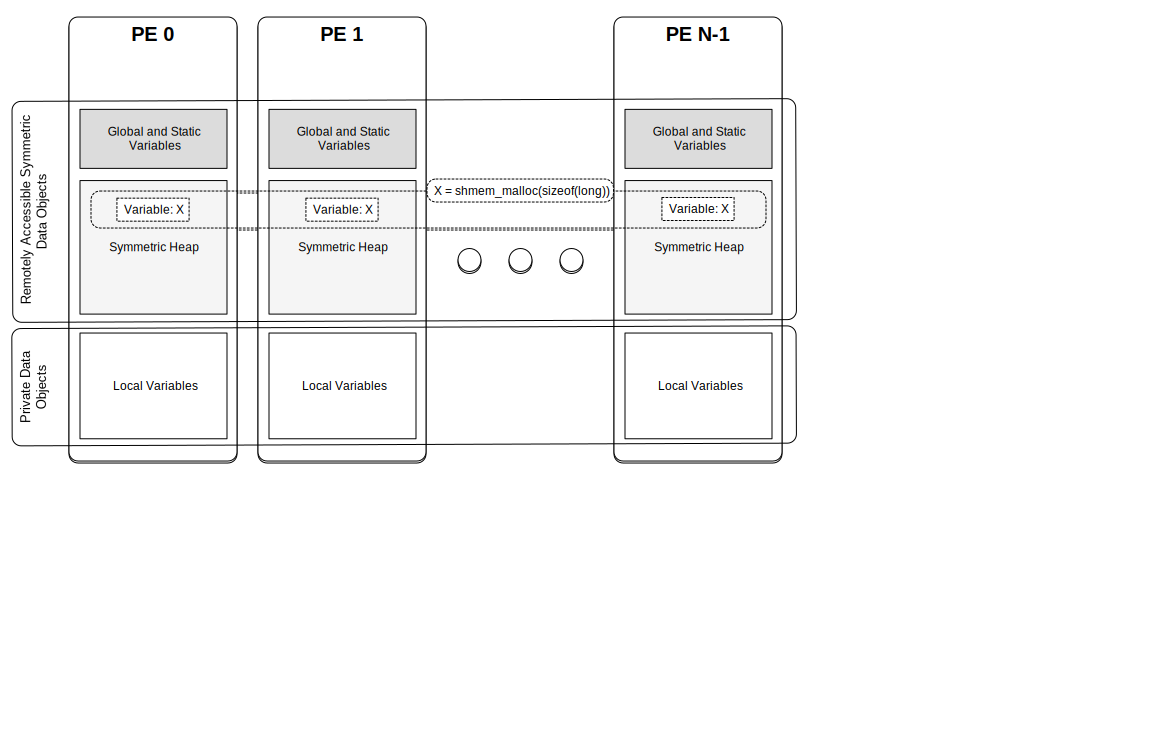
\includegraphics[width=0.95\textwidth]{figures/mem_model}      
\caption{\openshmem Memory Model}
\label{fig:mem_model}                                               
\end{figure}      
%
An \openshmem program consists of data objects that are private to each \ac{PE}
and data  objects that are remotely accessible by all \acp{PE}. Private data
objects are stored in the local memory of each \ac{PE} and can only be accessed
by the \ac{PE} itself; these data objects cannot be accessed by other \acp{PE}
via \openshmem routines. Private data objects follow the memory model of
\Cstd or \Fortran. Remotely accessible objects, however, can be accessed by
remote \acp{PE} using \openshmem routines.  Remotely accessible data objects are
called \emph{Symmetric Data Objects}.  Each symmetric data object has a
corresponding object with the same name, type, and size on all \acp{PE} where that object is
accessible via the \openshmem \ac{API}\footnote{For efficiency reasons,
the same offset (from an arbitrary memory address) for symmetric data
objects might be used on all \acp{PE}. Further discussion about symmetric heap
layout and implementation efficiency can be found in section
\ref{subsec:shfree}}.  (For the definition of what is accessible, see the
descriptions for \FUNC{shmem\_pe\_accessible} and \FUNC{shmem\_addr\_accessible}
in sections \ref{subsec:shmem_pe_accessible} and
\ref{subsec:shmem_addr_accessible}.) Symmetric data objects accessed via typed and
type-generic \openshmem interfaces are required to be naturally aligned based on their type
requirements and underlying architecture.  In \openshmem the following kinds of
data objects are symmetric:
%
\begin{itemize}
\item
  \begin{deprecate}
    \Fortran data objects in common blocks or with the \CTYPE{SAVE} attribute.
    These data objects must not be defined in a dynamic shared object (DSO).
  \end{deprecate}
\item Global and static \Cstd and \Cpp variables. These data objects must
  not  be defined in a DSO.
\item
  \begin{deprecate}
    \Fortran arrays allocated with \FUNC{shpalloc}
  \end{deprecate}
\item \Cstd and \Cpp data allocated by \openshmem memory management routines
  (Section~\ref{sec:memory_management})
\end{itemize}       

\openshmem dynamic memory allocation routines (\FUNC{shpalloc} and
\FUNC{shmem\_malloc}) allow collective allocation of \emph{Symmetric Data
Objects} on a special memory region called the \emph{Symmetric Heap}. The
Symmetric Heap is created during the execution of a program at a memory location
determined by the implementation. The Symmetric Heap may reside in different
memory regions on different \acp{PE}. Figure~\ref{fig:mem_model} shows how
\openshmem implements a \ac{PGAS} model using remotely accessible symmetric
objects and private data objects when executing an \openshmem program.
Symmetric data objects are stored on the symmetric heap or in the global/static
memory section of each \ac{PE}. 

\subsection{Atomicity Guarantees}\label{subsec:amo_guarantees}

\openshmem contains a number of routines that perform atomic operations on
symmetric data objects (Section \ref{sec:amo}).  These routines guarantee that
concurrent accesses to the same location by \openshmem atomic operations using
the same datatype will be exclusive.  However, they do not guarantee
exclusivity when concurrent accesses to the same location are performed using
\openshmem atomic operations using different datatypes, when non-atomic
\openshmem operations are used to access the given location, or when
non-\openshmem operations are performed on the given location.  The result in
such scenarios is undefined.

For example: during the execution of an atomic remote integer increment
operation on a symmetric variable \VAR{X}, no other \openshmem atomic operation
may access \VAR{X}.  After the increment, \VAR{X} will have increased its value
by \CONST{1} on the destination \ac{PE}, at which point other atomic operations
may then modify that \VAR{X}.  However, access to the symmetric object \VAR{X}
with non-atomic operations, such as one-sided \OPR{put} or \OPR{get} operations,
will invalidate the atomicity guarantees.


\section{Execution Model}\label{subsec:execution_model}
An \openshmem program consists of a set of \openshmem processes called \ac{PE}s
that execute in a \ac{SPMD}-like model where each \ac{PE} can take a different
execution path. For example, a \ac{PE} can be implemented using an OS
process.  The \ac{PE}s progress asynchronously, and can communicate/synchronize
via the \openshmem interfaces.  All \ac{PE}s in an \openshmem program should
start by calling the initialization routine  \FUNC{shmem\_init}
\footnote{\textbf{start\_pes} has been deprecated as of Specification 1.2}
before using any of the other \openshmem library routines.  An \openshmem
program finishes execution by returning from the main routine or when any PE
calls \FUNC{shmem\_global\_exit}. When returning from main, \openshmem must
complete all pending communication and release all the resources associated to
the library using an implicit collective synchronization across PEs. The user
has the option to call \FUNC{shmem\_finalize} (before returning from main) to
complete all pending communication and release all the \openshmem library
resources without terminating the program. Calling any \openshmem routine after
\FUNC{shmem\_finalize} leads to undefined behavior.

The \ac{PE}s of the \openshmem program are identified by unique integers.  The
identifiers are integers assigned in a monotonically increasing manner from zero
to the total number of \ac{PE}s minus 1. \ac{PE} identifiers are used for
\openshmem calls (e.g. to specify \OPR{put} or \OPR{get} routines on symmetric
data objects, collective synchronization calls) or to dictate a control flow for
\ac{PE}s using constructs of \Clang{} or \Fortran. The identifiers are fixed for
the life of the \openshmem program.

\subsection{Progress of \openshmem Operations}\label{subsec:progress}

The \openshmem model assumes that computation and communication are naturally
overlapped. \openshmem programs are expected to exhibit progression of
communication both with and without \openshmem calls. Consider a \ac{PE} that is
engaged in a computation with no \openshmem calls. Other \ac{PE}s should be able
to communicate (\OPR{put}, \OPR{get}, \OPR{collective}, \OPR{atomic}, etc) and
complete communication operations with that computationally-bound \ac{PE}
without that \ac{PE} issuing any explicit \openshmem calls. \openshmem
communication calls involving that \ac{PE} should progress regardless of when
that \ac{PE} next engages in an \openshmem call.

\textbf{Note to implementors:}
\begin{itemize}
  \item An \openshmem implementation for hardware that does not provide
      asynchronous communication capabilities may require a software progress
      thread in order to process remotely-issued communication requests without
      explicit program calls to the \openshmem library.  
  \item High performance implementations of \openshmem are expected to leverage
      hardware offload capabilities and provide asynchronous one-sided
      communication without software assistance.
  \item Implementations should avoid deferring the execution of one-sided
      operations until a synchronization point where data is known to be
      available. High-quality implementations should attempt asynchronous delivery
      whenever possible, for performance reasons. Additionally, the \openshmem
      community discourages releasing \openshmem implementations that do not
      provide asynchronous one-sided operations, as these have very limited
      performance value for \openshmem programs.
\end{itemize}

\subsection{Atomicity Guarantees}\label{sec:amo_guarantees}

\openshmem contains a number of routines that operate on symmetric data
atomically (Section \ref{sec:amo}).  These routines guarantee that accesses by
\openshmem's atomic operations with the same datatype will be exclusive, but do not guarantee
exclusivity in combination with other routines, either inside \openshmem or
outside.

For example: during the execution of an atomic remote integer increment
operation on a symmetric variable \VAR{X}, no other \openshmem atomic operation
may access \VAR{X}.  After the increment, \VAR{X} will have increased its value
by \CONST{1} on the destination \ac{PE}, at which point other atomic operations
may then modify that \VAR{X}.  However, access to the symmetric object \VAR{X}
with non-atomic operations, such as one-sided \OPR{put} or \OPR{get} operations,
will \OPR{invalidate} the atomicity guarantees.


\section{Language Bindings and Conformance}\label{subsec:bindings}
\openshmem provides ISO \Cstd language bindings. Any implementation that
provides \Cstd bindings can claim conformance to the specification. The
\openshmem header file \HEADER{shmem.h} for \Cstd must contain only the
interfaces and constant names defined in this specification.

\openshmem \acp{API} can be implemented as either routines or macros. However,
implementing the interfaces using macros is strongly discouraged as this could
severely limit the use of external profiling tools and high-level compiler
optimizations. An \openshmem program should avoid defining routine names,
variables, or identifiers with the prefix \shmemprefix, \shmemprefixC, or with
\openshmem \ac{API} names.

All \openshmem extension \acp{API} that are not part of this specification must
be defined in the \HEADER{shmemx.h} include file for language bindings. This
header file must exist, even if no extensions are provided. Any extensions
shall use the \FUNC{shmemx\_} prefix for all routine, variable, and constant
names.


\section{Library Constants}\label{subsec:library_constants}
\TableIndex{Library Constants}
\TableIndex{Constants}

The \openshmem library provides a set of compile-time constants that may
be used to specify options to API routines, provide implementation-specific
parameters, or return information about the implementation.
All constants that start with \CONST{\_SHMEM\_*} are deprecated,
but provided for backwards compatibility.

\begin{longtable}{|p{0.45\textwidth}|p{0.5\textwidth}|}
\hline
\textbf{Constant} & \textbf{Description}
\tabularnewline \hline
\endhead
%%
\LibConstDecl{SHMEM\_THREAD\_SINGLE} &
The \openshmem thread support level which specifies that the program
must not be multithreaded.
See Section~\ref{subsec:thread_support} for more detail about its use.
\tabularnewline \hline
%%
\LibConstDecl{SHMEM\_THREAD\_FUNNELED} &
The \openshmem thread support level which specifies that the program
may be multithreaded but must ensure that only the main thread invokes
the \openshmem interfaces.
See Section~\ref{subsec:thread_support} for more detail about its use.
\tabularnewline \hline
%%
\LibConstDecl{SHMEM\_THREAD\_SERIALIZED} &
The \openshmem thread support level which specifies that the program
may be multithreaded but must ensure that the \openshmem interfaces
are not invoked concurrently by multiple threads.
See Section~\ref{subsec:thread_support} for more detail about its use.
\tabularnewline \hline
%%
\LibConstDecl{SHMEM\_THREAD\_MULTIPLE} &
The \openshmem thread support level which specifies that the program
may be multithreaded and any thread may invoke the \openshmem interfaces.
See Section~\ref{subsec:thread_support} for more detail about its use.
\tabularnewline \hline
%%
\color{Green}
\LibConstDecl{SHMEM\_TEAM\_NUM\_CONTEXTS} &
\color{Green}
The bitwise flag which specifies that a team creation routine should use the
\VAR{num\_contexts} member of the provided
\CTYPE{shmem\_team\_config\_t} configuration parameter as a request.
See Sections~\ref{subsec:shmem_team_config_t} and
\ref{subsec:shmem_team_split_strided} for more detail about its use.
\tabularnewline \hline
%%
\color{Green}
\LibConstDecl{SHMEM\_TEAM\_NULL} &
\color{Green}
Predefined constant that can be compared against handles of type
\CTYPE{shmem\_team\_t} to determine if they refer to a valid team.
See Section~\ref{subsec:team} for more detail about its use.
\tabularnewline \hline
%%
\LibConstDecl{SHMEM\_CTX\_INVALID} &
A value corresponding to an invalid communication context.
This value can be used to initialize or update context handles to indicate
that they do not reference a valid context.
When managed in this way, applications can use an equality comparison
to test whether a given context handle references a valid context.
See Section~\ref{sec:ctx} for more detail about its use.
\tabularnewline \hline
%%
\LibConstDecl{SHMEM\_CTX\_SERIALIZED} &
The context creation option which specifies that the given context
is shareable but will not be used by multiple threads concurrently.
See Section~\ref{subsec:shmem_ctx_create} for more detail about its use.
\tabularnewline \hline
%%
\LibConstDecl{SHMEM\_CTX\_PRIVATE} &
The context creation option which specifies that the given context
will be used only by the thread that created it.
See Section~\ref{subsec:shmem_ctx_create} for more detail about its use.
\tabularnewline \hline
%%
\LibConstDecl{SHMEM\_CTX\_NOSTORE} &
The context creation option which specifies that quiet and fence operations
performed on the given context are not required to enforce completion and
ordering of memory store operations.
See Section~\ref{subsec:shmem_ctx_create} for more detail about its use.
\tabularnewline \hline
%%
\LibConstDecl{SHMEM\_SYNC\_VALUE}
\begin{DeprecateBlock}
  \LibConstDecl{\_SHMEM\_SYNC\_VALUE}
  \LibConstDecl[\Fortran]{SHMEM\_SYNC\_VALUE}
\end{DeprecateBlock}
&
The value used to initialize the elements of \VAR{pSync} arrays.
The value of this constant is implementation specific.
See Section~\ref{subsec:coll} for more detail about its use.
\tabularnewline \hline
%%
\LibConstDecl{SHMEM\_SYNC\_SIZE}
\begin{DeprecateBlock}
  \LibConstDecl[\Fortran]{SHMEM\_SYNC\_SIZE}
\end{DeprecateBlock}
&
Length of a work array that can be used with any SHMEM collective
communication operation.
Work arrays sized for specific operations may consume less memory.
The value of this constant is implementation specific.
See Section~\ref{subsec:coll} for more detail about its use.
\tabularnewline \hline
%%
\LibConstDecl{SHMEM\_BCAST\_SYNC\_SIZE}
\begin{DeprecateBlock}
  \LibConstDecl{\_SHMEM\_BCAST\_SYNC\_SIZE}
  \LibConstDecl[\Fortran]{SHMEM\_BCAST\_SYNC\_SIZE}
\end{DeprecateBlock}
&
Length of the \VAR{pSync} arrays needed for broadcast routines. The value
of this constant is implementation specific.
See Section~\ref{subsec:shmem_broadcast} for more detail about its use.
\tabularnewline \hline
%%
\LibConstDecl{SHMEM\_REDUCE\_SYNC\_SIZE}
\begin{DeprecateBlock}
  \LibConstDecl{\_SHMEM\_REDUCE\_SYNC\_SIZE}
  \LibConstDecl[\Fortran]{SHMEM\_REDUCE\_SYNC\_SIZE}
\end{DeprecateBlock}
&
Length of the work arrays needed for reduction routines.
The value of this constant is implementation specific.
See Section~\ref{subsec:shmem_reductions} for more detail about its use.
\tabularnewline \hline
%%
\LibConstDecl{SHMEM\_BARRIER\_SYNC\_SIZE}
\begin{DeprecateBlock}
  \LibConstDecl{\_SHMEM\_BARRIER\_SYNC\_SIZE}
  \LibConstDecl[\Fortran]{SHMEM\_BARRIER\_SYNC\_SIZE}
\end{DeprecateBlock}
&
Length of the work array needed for barrier routines.
The value of this constant is implementation specific.
See Section~\ref{subsec:shmem_barrier} for more detail about its use.

\tabularnewline \hline
%%
\LibConstDecl{SHMEM\_COLLECT\_SYNC\_SIZE}
\begin{DeprecateBlock}
  \LibConstDecl{\_SHMEM\_COLLECT\_SYNC\_SIZE}
  \LibConstDecl[\Fortran]{SHMEM\_COLLECT\_SYNC\_SIZE}
\end{DeprecateBlock}
&
Length of the work array needed for collect routines.
The value of this constant is implementation specific.
See Section~\ref{subsec:shmem_collect} for more detail about its use.
\tabularnewline \hline
%%
\LibConstDecl{SHMEM\_ALLTOALL\_SYNC\_SIZE}
\begin{DeprecateBlock}
  \LibConstDecl[\Fortran]{SHMEM\_ALLTOALL\_SYNC\_SIZE}
\end{DeprecateBlock}
&
Length of the work array needed for \FUNC{shmem\_alltoall} routines.
The value of this constant is implementation specific.
See Section~\ref{subsec:shmem_alltoall} for more detail about its use.
\tabularnewline \hline
%%
\LibConstDecl{SHMEM\_ALLTOALLS\_SYNC\_SIZE}
\begin{DeprecateBlock}
  \LibConstDecl[\Fortran]{SHMEM\_ALLTOALLS\_SYNC\_SIZE}
\end{DeprecateBlock}
&
Length of the work array needed for \FUNC{shmem\_alltoalls} routines.
The value of this constant is implementation specific.
See Section~\ref{subsec:shmem_alltoalls} for more detail about its use.
\tabularnewline \hline
%%
\LibConstDecl{SHMEM\_REDUCE\_MIN\_WRKDATA\_SIZE}
\begin{DeprecateBlock}
  \LibConstDecl{\_SHMEM\_REDUCE\_MIN\_WRKDATA\_SIZE}
  \LibConstDecl[\Fortran]{SHMEM\_REDUCE\_MIN\_WRKDATA\_SIZE}
\end{DeprecateBlock}
&
Minimum length of work arrays used in various collective routines.
\tabularnewline \hline
%%
\LibConstDecl{SHMEM\_MAJOR\_VERSION}
\begin{DeprecateBlock}
  \LibConstDecl{\_SHMEM\_MAJOR\_VERSION}
  \LibConstDecl[\Fortran]{SHMEM\_MAJOR\_VERSION}
\end{DeprecateBlock}
&
Integer representing the major version of \openshmem Specification in use.
\tabularnewline \hline
%%
\LibConstDecl{SHMEM\_MINOR\_VERSION}
\begin{DeprecateBlock}
  \LibConstDecl{\_SHMEM\_MINOR\_VERSION}
  \LibConstDecl[\Fortran]{SHMEM\_MINOR\_VERSION}
\end{DeprecateBlock}
&
Integer representing the minor version of \openshmem Specification in use.
\tabularnewline \hline
%%
\LibConstDecl{SHMEM\_MAX\_NAME\_LEN}
\begin{DeprecateBlock}
  \LibConstDecl{\_SHMEM\_MAX\_NAME\_LEN}
  \LibConstDecl[\Fortran]{SHMEM\_MAX\_NAME\_LEN}
\end{DeprecateBlock}
&
Integer representing the maximum length of \CONST{SHMEM\_VENDOR\_STRING}.
\tabularnewline \hline
%%
\LibConstDecl{SHMEM\_VENDOR\_STRING}
\begin{DeprecateBlock}
  \LibConstDecl{\_SHMEM\_VENDOR\_STRING}
  \LibConstDecl[\Fortran]{SHMEM\_VENDOR\_STRING}
\end{DeprecateBlock}
&
String representing vendor defined information of size at most
\CONST{SHMEM\_MAX\_NAME\_LEN}.
In \CorCpp{}, the string is terminated by a null character.  In \Fortran, the
string of size less than \CONST{SHMEM\_MAX\_NAME\_LEN} is padded with blank
characters up to size \CONST{SHMEM\_MAX\_NAME\_LEN}.
\tabularnewline \hline
%%
\LibConstDecl{SHMEM\_CMP\_EQ}
\begin{DeprecateBlock}
  \LibConstDecl{\_SHMEM\_CMP\_EQ}
  \LibConstDecl[\Fortran]{SHMEM\_CMP\_EQ}
\end{DeprecateBlock}
&
An integer constant expression corresponding to the
``equal to'' comparison operation.
See Section~\ref{subsec:p2p_intro} for more detail about its use.
\tabularnewline \hline
%%
\LibConstDecl{SHMEM\_CMP\_NE}
\begin{DeprecateBlock}
  \LibConstDecl{\_SHMEM\_CMP\_NE}
  \LibConstDecl[\Fortran]{SHMEM\_CMP\_NE}
\end{DeprecateBlock}
&
An integer constant expression corresponding to the
``not equal to'' comparison operation.
See Section~\ref{subsec:p2p_intro} for more detail about its use.
\tabularnewline \hline
%%
\LibConstDecl{SHMEM\_CMP\_LT}
\begin{DeprecateBlock}
  \LibConstDecl{\_SHMEM\_CMP\_LT}
  \LibConstDecl[\Fortran]{SHMEM\_CMP\_LT}
\end{DeprecateBlock}
&
An integer constant expression corresponding to the
``less than'' comparison operation.
See Section~\ref{subsec:p2p_intro} for more detail about its use.
\tabularnewline \hline
%%
\LibConstDecl{SHMEM\_CMP\_LE}
\begin{DeprecateBlock}
  \LibConstDecl{\_SHMEM\_CMP\_LE}
  \LibConstDecl[\Fortran]{SHMEM\_CMP\_LE}
\end{DeprecateBlock}
&
An integer constant expression corresponding to the
``less than or equal to'' comparison operation.
See Section~\ref{subsec:p2p_intro} for more detail about its use.
\tabularnewline \hline
%%
\LibConstDecl{SHMEM\_CMP\_GT}
\begin{DeprecateBlock}
  \LibConstDecl{\_SHMEM\_CMP\_GT}
  \LibConstDecl[\Fortran]{SHMEM\_CMP\_GT}
\end{DeprecateBlock}
&
An integer constant expression corresponding to the
``greater than'' comparison operation.
See Section~\ref{subsec:p2p_intro} for more detail about its use.
\tabularnewline \hline
%%
\LibConstDecl{SHMEM\_CMP\_GE}
\begin{DeprecateBlock}
  \LibConstDecl{\_SHMEM\_CMP\_GE}
  \LibConstDecl[\Fortran]{SHMEM\_CMP\_GE}
\end{DeprecateBlock}
&
An integer constant expression corresponding to the
``greater than or equal to'' comparison operation.
See Section~\ref{subsec:p2p_intro} for more detail about its use.
\tabularnewline \hline
%%
\end{longtable}


\section{Environment Variables }\label{subsec:environment_variables}
The \openshmem specification provides a set of environment variables that allows
users to configure the \openshmem implementation, and receive information about
the implementation. The implementations of the specification are free to define
additional variables. Currently, the specification defines four environment
variables. All environment variables that start with \VAR{SMA\_*} are
deprecated, but currently supported for backwards compatibility.

\medskip{}

\begin{tabular}{|l|l|l|}
\hline 
Variable & Value & Purpose\tabularnewline
\hline 
\hline 
\texttt{SHMEM\_VERSION} & any & print the library version at
start-up\tabularnewline
\hline 
\texttt{SHMEM\_INFO} & any & print helpful text about all these environment
variables\tabularnewline
\hline 
\texttt{SHMEM\_SYMMETRIC\_SIZE} & non-negative integer & number of bytes to
allocate for symmetric heap\tabularnewline
\hline 
\texttt{SHMEM\_DEBUG} & any & enable debugging messages\tabularnewline
\hline 
\end{tabular}

\medskip{}





\clearpage



\section{OpenSHMEM Library API}\label{sec:openshmem_library_api}

\subsection{Library Setup, Exit, and Query Routines}
The library setup and query interfaces that initialize and monitor the parallel
environment of the \ac{PE}s.

\subsubsection{\textbf{SHMEM\_INIT}}\label{subsec:shmem_init}
\apisummary{
    A collective operation that allocates and initializes the resources used by
    the \openshmem library.
}

\begin{apidefinition}

\begin{Csynopsis}
void @\FuncDecl{shmem\_init}@(void);
\end{Csynopsis}

\begin{apiarguments}
    \apiargument{None.}{}{}
\end{apiarguments}

\apidescription{
    \FUNC{shmem\_init} allocates and initializes resources used by the \openshmem
    library. It is a collective operation that all \acp{PE} must call before any
    other \openshmem routine may be called, except \FUNC{shmem\_query\_initialized} 
    which checks the current initialized state of the library. At the end of the 
    \openshmem program which it initialized, the call to \FUNC{shmem\_init} must 
    be matched with a call to \FUNC{shmem\_finalize}.

    The \FUNC{shmem\_init} and \FUNC{shmem\_init\_thread} initialization
    routines may be called multiple times within an \openshmem program. A
    corresponding call to \FUNC{shmem\_finalize} must be made for each call to
    an \openshmem initialization routine. The \openshmem library must not be
    finalized until after the last call to \FUNC{shmem\_finalize} and may be
    re-initialized with a subsequent call to an initialization routine.

}

\apireturnvalues{
    None.
}

\begin{DeprecateBlock}
\apinotes{
    As of \openshmem[1.2], the use of \FUNC{start\_pes} has been
    deprecated and calls to it should be replaced with calls to \FUNC{shmem\_init}.
    While support for \FUNC{start\_pes} is still required in \openshmem libraries,
    users are encouraged to use \FUNC{shmem\_init}. An important difference between
    \FUNC{shmem\_init} and \FUNC{start\_pes} is that every call to
    \FUNC{shmem\_init} within a program must be matched with a call to \FUNC{shmem\_finalize}.
    In the case of \FUNC{start\_pes}, any subsequent calls to \FUNC{start\_pes} after the
    first one results in a no-op.
}
\end{DeprecateBlock}

\begin{apiexamples}

\apicexample
    {The following \FUNC{shmem\_init} example is for \Cstd[11] programs:}
    {example_code/shmem_init_example.c}
    {}

\end{apiexamples}

\end{apidefinition}


\subsubsection{\textbf{SHMEM\_MY\_PE}}\label{subsec:shmem_my_pe}
\apisummary{
    Returns the number of the calling \ac{PE}.
}

\begin{apidefinition}

\begin{Csynopsis}
int shmem_my_pe(void);
\end{Csynopsis}

\begin{Fsynopsis}
INTEGER SHMEM_MY_PE, ME
ME = SHMEM_MY_PE()
\end{Fsynopsis}

\begin{apiarguments}
    \apiargument{None.}{}{}
\end{apiarguments}

\apidescription{
    This routine returns the \ac{PE} number of the calling \ac{PE}.  It accepts no
    arguments.  The result is an integer between \CONST{0} and \VAR{npes} -
    \CONST{1}, where \VAR{npes} is the total number of \ac{PE}s executing the
    current program.
}

\apireturnvalues{
    Integer - Between \CONST{0} and \VAR{npes} - \CONST{1}
}

\apinotes{
    Each \ac{PE} has a unique number or identifier. As of \openshmem Specification
    1.2 the use of \FUNC{\_my\_pe} has been deprecated. Although \openshmem
    libraries are required to support the call, users are encouraged to use
    \FUNC{shmem\_my\_pe} instead.  The behavior and signature  of the routine
    \FUNC{shmem\_my\_pe} remains unchanged from the deprecated \FUNC{\_my\_pe}
    version.
}

\end{apidefinition}


\subsubsection{\textbf{SHMEM\_N\_PES}}\label{subsec:shmem_n_pes}
\apisummary{
    Returns the number of \ac{PE}s running in a program.
}

\begin{apidefinition}

\begin{Csynopsis}
int shmem_n_pes(void);
\end{Csynopsis}

\begin{Fsynopsis}
INTEGER SHMEM_N_PES, N_PES
N_PES = SHMEM_N_PES()
N_PES = NUM_PES()
\end{Fsynopsis}

\begin{apiarguments}
    \apiargument{None.}{}{}
\end{apiarguments}

\apidescription{
    The routine returns the number of \ac{PE}s running the program.
}

\apireturnvalues{
    Integer -  Number of \ac{PE}s running the \openshmem program.
}

\apinotes{
    As of \openshmem Specification 1.2 the use of \FUNC{\_num\_pes} has been
    deprecated. Although \openshmem libraries are required to support the call,
    users are encouraged to use \FUNC{shmem\_n\_pes} instead.
}

\begin{apiexamples}

\apicexample
    {The following \FUNC{shmem\_n\_pes} example is for \CorCpp{} programs:}
    {./example_code/shmem_npes_example.c}
    {}

\end{apiexamples}

\end{apidefinition}


\subsubsection{\textbf{SHMEM\_FINALIZE}}\label{subsec:shmem_finalize}
\apisummary{
    A collective operation that releases all resources used by the \openshmem
    library.  This only terminates the \openshmem portion of a program, not the
    entire program.
}

\begin{apidefinition}

\begin{Csynopsis}
void @\FuncDecl{shmem\_finalize}@(void);
\end{Csynopsis}

\begin{apiarguments}
    \apiargument{None.}{}{}
\end{apiarguments}

\apidescription{
    \FUNC{shmem\_finalize} is a collective operation that ends the \openshmem
    portion of a program previously initialized by \FUNC{shmem\_init} or \FUNC{shmem\_init\_thread} and
    releases all resources used by the \openshmem library. This collective
    operation requires all \acp{PE} to participate in the call. There is an
    implicit global barrier in \FUNC{shmem\_finalize} to ensure that pending
    communications are completed and that no resources are released until all
    \acp{PE} have entered \FUNC{shmem\_finalize}.
    This routine destroys all shareable contexts.  The user is
    responsible for destroying all contexts with the
    \CONST{SHMEM\_CTX\_PRIVATE} option enabled prior to calling this routine;
    otherwise, the behavior is undefined.
    \FUNC{shmem\_finalize} must be
    the last \openshmem library call encountered in the \openshmem portion of a
    program. A call to \FUNC{shmem\_finalize} will release all resources
    initialized by a corresponding call to \FUNC{shmem\_init} or \FUNC{shmem\_init\_thread}. All processes
    that represent the \acp{PE} will still exist after the
    call to \FUNC{shmem\_finalize} returns, but they will no longer have access
    to resources that have been released.
}

\apireturnvalues{
    None.
}

\apinotes{
    \FUNC{shmem\_finalize} releases all resources used by the \openshmem library
    including the symmetric memory heap and pointers initiated by
    \FUNC{shmem\_ptr}. This collective operation requires all \acp{PE} to
    participate in the call, not just a subset of the \acp{PE}. The
    non-\openshmem portion of a program may continue after a call to
    \FUNC{shmem\_finalize} by all \acp{PE}.
}

\begin{apiexamples}

\apicexample
    {The following finalize example is for \Cstd[11] programs:}
    {./example_code/shmem_finalize_example.c}
    {}

\end{apiexamples}

\end{apidefinition}


\subsubsection{\textbf{SHMEM\_GLOBAL\_EXIT}}\label{subsec:shmem_global_exit}
\apisummary{
    A routine that allows any \ac{PE} to force termination of an entire program.
}

\begin{apidefinition}

\begin{C11synopsis}
_Noreturn void shmem_global_exit(int status);
\end{C11synopsis}

\begin{Csynopsis}
void shmem_global_exit(int status);
\end{Csynopsis}

\begin{Fsynopsis}
INTEGER STATUS
CALL SHMEM_GLOBAL_EXIT(status)
\end{Fsynopsis}

\begin{apiarguments}
    \apiargument{IN}{status}{The exit status from the main program.}
\end{apiarguments}

\apidescription{
    \FUNC{shmem\_global\_exit} is a non-collective routine that allows any one
    \ac{PE} to force termination of an \openshmem program for all \acp{PE},
    passing an exit status to the execution environment. This routine terminates
    the entire program, not just the \openshmem portion.  When any \ac{PE} calls
    \FUNC{shmem\_global\_exit}, it results in the immediate notification to all
    \acp{PE} to terminate.  \FUNC{shmem\_global\_exit} flushes I/O and releases
    resources in accordance with C/C++/Fortran language requirements for normal
    program termination. If more than one \ac{PE} calls
    \FUNC{shmem\_global\_exit}, then the exit status returned to the environment
    shall be one of the values passed to \FUNC{shmem\_global\_exit} as the
    status argument.  There is no return to the caller of
    \FUNC{shmem\_global\_exit}; control is returned from the \openshmem program
    to the execution environment for all \acp{PE}.
}

\apireturnvalues{
    None.
}


\apinotes{ 
    \FUNC{shmem\_global\_exit} may be used in situations where one or more
    \acp{PE} have determined that the program has completed and/or should
    terminate early.  Accordingly, the integer status argument can be used to
    pass any information about the nature of the exit, e.g an encountered error
    or a found solution.  Since \FUNC{shmem\_global\_exit} is a non-collective
    routine, there is no implied synchronization, and all \acp{PE} must
    terminate regardless of their current execution state. While I/O must be
    flushed for standard language I/O calls from C/C++/Fortran, it is
    implementation dependent as to how I/O done by other means (e.g. third
    party I/O libraries) is handled. Similarly, resources are released
    according to C/C++/Fortran standard language requirements, but this may not
    include all resources allocated for the \openshmem program. However, a
    quality implementation will make a best effort to flush all I/O and clean
    up all resources.
}

\begin{apiexamples}

\apicexample
    {}
    {./example_code/shmem_global_exit_example.c}
    {}

\end{apiexamples}

\end{apidefinition}


\subsubsection{\textbf{SHMEM\_PE\_ACCESSIBLE}}\label{subsec:shmem_pe_accessible}
\apisummary{
    Determines whether a \ac{PE} is accessible via \openshmem's data transfer
    routines.
}

\begin{apidefinition}

\begin{Csynopsis}
int shmem_pe_accessible(int pe);
\end{Csynopsis}

\begin{Fsynopsis}
LOGICAL LOG, SHMEM_PE_ACCESSIBLE
INTEGER pe
LOG = SHMEM_PE_ACCESSIBLE(pe)
\end{Fsynopsis}

\begin{apiarguments}
    \apiargument{IN}{pe}{Specific \ac{PE} to be checked for accessibility from
    the local \ac{PE}.}
\end{apiarguments}

\apidescription{
    \FUNC{shmem\_pe\_accessible} is a query routine that indicates whether a
    specified \ac{PE} is accessible via \openshmem from the local \ac{PE}. The
    \FUNC{shmem\_pe\_accessible} routine returns a value indicating whether the remote
    \ac{PE} is a process running from the same executable file as the local
    \ac{PE}, thereby indicating whether full support for symmetric data objects,
    which may reside in either static memory or the symmetric heap, is available.
}

\apireturnvalues{
    \CorCpp: The return value is 1 if the specified \ac{PE} is a valid remote \ac{PE}
    for \openshmem routines; otherwise, it is 0.

    \Fortran: The return value is \CONST{.TRUE.} if the specified \ac{PE} is a valid
    remote \ac{PE} for \openshmem routines; otherwise, it is \CONST{.FALSE.}.
}

\apinotes{
    This routine may be particularly useful for hybrid programming with other
    communication libraries (such as \ac{MPI}) or parallel languages.  For
    example, when an \ac{MPI} job uses \ac{MPMD} mode, multiple executable
    \ac{MPI} programs are executed as part of the same MPI job.  In such cases,
    \openshmem support may only be available between processes running from the
    same executable file.  In addition, some environments may allow a hybrid
    job to span multiple network partitions.  In such scenarios, \openshmem
    support may only be available between \acp{PE} within the same partition.
}

\end{apidefinition}


\subsubsection{\textbf{SHMEM\_ADDR\_ACCESSIBLE}}\label{subsec:shmem_addr_accessible}
\apisummary{
    Determines whether an address is accessible via OpenSHMEM data transfer
    routines from the specified  remote \ac{PE}.
}
\index{SHMEM\_ADDR\_ACCESSIBLE}

\begin{apidefinition}

\begin{Csynopsis}
int shmem_addr_accessible(const void *addr, int pe);
\end{Csynopsis}

\begin{Fsynopsis}
LOGICAL LOG, SHMEM_ADDR_ACCESSIBLE
INTEGER pe
LOG = SHMEM_ADDR_ACCESSIBLE(addr, pe)
\end{Fsynopsis}

\begin{apiarguments}
    \apiargument{IN}{addr}{Data object on the local \ac{PE}.}
    \apiargument{IN}{pe}{Integer id of a remote \ac{PE}.}
\end{apiarguments}

\apidescription{
    \FUNC{shmem\_addr\_accessible} is a query routine that indicates whether a local
    address is accessible via \openshmem routines from the specified remote \ac{PE}. 
    
    This routine verifies that the data object is symmetric and accessible with
    respect to a remote \ac{PE} via \openshmem  data  transfer routines.  The
    specified address \VAR{addr} is a data object on the local \ac{PE}. 
    
    This routine may be particularly useful for hybrid programming with other
    communication libraries (such as \ac{MPI}) or parallel languages.  For
    example, in SGI Altix series systems, for multiple executable MPI programs that
    use \openshmem routines, it is important to note that static memory, such as a
    \Fortran common block or \Cstd global variable, is symmetric between
    processes running from the same executable file, but is not symmetric between
    processes running from different executable files.  Data allocated from the
    symmetric heap (\FUNC{shmem\_malloc} or \FUNC{shpalloc}) is symmetric across the
    same or different executable files.
}

\apireturnvalues{		
    \CorCpp: The  return value is \CONST{1} if \VAR{addr} is a symmetric data object
    and accessible via \openshmem routines from the specified remote \ac{PE};
    otherwise, it is \CONST{0}.
    
    \Fortran: The return value is \CONST{.TRUE.} if \VAR{addr} is a symmetric data
    object and accessible via \openshmem routines from the specified remote \ac{PE};
    otherwise, it is \CONST{.FALSE.}.
}
		
\apinotes{
    None.
}

\end{apidefinition}


\subsubsection{\textbf{SHMEM\_PTR}}\label{subsec:shmem_ptr}
\apisummary{
    Returns a local pointer to a symmetric data object on the specified \ac{PE} in the world team.
}

\begin{apidefinition}

\begin{Csynopsis}
void *@\FuncDecl{shmem\_ptr}@(const void *dest, int pe);
\end{Csynopsis}

\begin{apiarguments}
\apiargument{IN}{dest}{The symmetric address of the remotely accessible data
    object to be referenced.}
\apiargument{IN}{pe}{An integer that indicates the \ac{PE} number on which \dest{} is to
    be accessed.}
\end{apiarguments}

\apidescription{
    \FUNC{shmem\_ptr} returns an address that may be used to directly reference
    \dest{} on the specified \ac{PE} in the world team.  This address can be
    assigned to a pointer.  After that, ordinary loads and stores to \dest{} may
    be performed.  The address returned by \FUNC{shmem\_ptr} is a local address
    to a remotely accessible data object.  Providing this address to an argument
    of an \openshmem routine that requires a symmetric address results in
    undefined behavior.

    The \FUNC{shmem\_ptr} routine can provide efficient means to accomplish
    communication, for example when a sequence of reads and writes to a data
    object on a remote \ac{PE} does not match the access pattern provided in an
    \openshmem data transfer routine like \FUNC{shmem\_put} or
    \FUNC{shmem\_iget}.
}

\apireturnvalues{
    A local pointer to the remotely accessible \dest{} data object is returned
    when it can be accessed using memory loads and stores.  Otherwise, a null
    pointer is returned.
}

\apinotes{
    When calling \FUNC{shmem\_ptr}, \dest{} is the address of the referenced
    symmetric data object on the calling \ac{PE}.
}

\begin{apiexamples}

\apicexample
    {In the following \Cstd[11] example, \ac{PE} 0 uses the \FUNC{shmem\_ptr}
    routine to query a pointer and directly access the \VAR{dest} array on
    \ac{PE} 1:}
    {./example_code/shmem_ptr_example.c}
    {}

\end{apiexamples}

\end{apidefinition}


\subsubsection{\textbf{SHMEM\_INFO\_GET\_VERSION}}\label{subsec:shmem_info_get_version}
\apisummary{
    Returns the major and minor version of the library implementation.
}

\begin{apidefinition}

\begin{Csynopsis}
void @\FuncDecl{shmem\_info\_get\_version}@(int *major, int *minor);
\end{Csynopsis}

\begin{Fsynopsis}
INTEGER MAJOR, MINOR
CALL @\FuncDecl{SHMEM\_INFO\_GET\_VERSION}@(MAJOR, MINOR)
\end{Fsynopsis}

\begin{apiarguments}
    \apiargument{OUT}{major}{The major version of the \openshmem Specification in use.}
    \apiargument{OUT}{minor}{The minor version of the \openshmem Specification in use.}
\end{apiarguments}

\apidescription{
    This routine returns the major and minor version of the \openshmem Specification
    in use.  For a given library implementation, the major and minor version
    returned by these calls are consistent with the library constants
    \CONST{SHMEM\_MAJOR\_VERSION} and \CONST{SHMEM\_MINOR\_VERSION}.
}

\apireturnvalues{
    None.
}

\apinotes{
    None. 
}

\end{apidefinition}


\subsubsection{\textbf{SHMEM\_INFO\_GET\_NAME}}\label{subsec:shmem_info_get_name}
\apisummary{
    This routine returns the vendor defined name string that is consistent
    with the library constant \CONST{SHMEM\_VENDOR\_STRING}.
}

\begin{apidefinition}

\begin{Csynopsis}
void @\FuncDecl{shmem\_info\_get\_name}@(char *name);
\end{Csynopsis}

\begin{Fsynopsis}
CHARACTER *(*)NAME
CALL @\FuncDecl{SHMEM\_INFO\_GET\_NAME}@(NAME)
\end{Fsynopsis}

\begin{apiarguments}
    \apiargument{OUT}{name}{The vendor defined string.}
\end{apiarguments}

\apidescription{
    This routine returns the vendor defined name string of size defined by
    the library constant \CONST{SHMEM\_MAX\_NAME\_LEN}. The program calling
    this function provides the \VAR{name} memory buffer of at least size
    \CONST{SHMEM\_MAX\_NAME\_LEN}. The implementation copies the vendor defined
    string of size at most \CONST{SHMEM\_MAX\_NAME\_LEN} to \VAR{name}. In
    \CorCpp, the string is terminated by a null character.  In \Fortran,
    the string of size less than \CONST{SHMEM\_MAX\_NAME\_LEN} is padded with
    blank characters up to size \CONST{SHMEM\_MAX\_NAME\_LEN}. If the
    \VAR{name} memory buffer is provided with size less than
    \CONST{SHMEM\_MAX\_NAME\_LEN}, behavior is undefined. For a given library
    implementation, the vendor string returned is consistent with the library
    constant \CONST{SHMEM\_VENDOR\_STRING}.
}

\apireturnvalues{ 
    None. 
}

\apinotes{ 
    None. 
}

\end{apidefinition}



\subsection{Memory Management Routines}
\openshmem provides a set of \ac{API}s for managing the symmetric heap. The
\ac{API}s allow one to dynamically allocate, deallocate, reallocate and align
symmetric data objects in the symmetric heap, in \Clang{} and \Fortran.



\clearpage %%%%%%%%%%%%%%%%%%%%%%%%%%%%%%%%%%%%%%%%%%%%%%%%%%%%%%%%%%%%

\appendix

%defining pagestyle for annex
\pagestyle{fancy}
\fancyhf{}
\fancyhead[L]{\leftmark}
\fancyhead[R]{\thepage}
\renewcommand{\headrulewidth}{0pt}
\renewcommand{\thesection}{\thesectionOrig}




\chapter{Writing OpenSHMEM Programs}
\section*{Incorporating OpenSHMEM into Programs}\label{sec:writing_programs}

The following section describes how to write a ``Hello World" \openshmem program.
To write a ``Hello World" \openshmem program, the user must:

\begin{itemize}
\item Include the header file \HEADER{shmem.h} for \Cstd.
\item Add the initialization call \hyperref[subsec:shmem_init]{\FUNC{shmem\_init}}.
\item Use \openshmem calls to query the local \ac{PE} number
    (\hyperref[subsec:shmem_my_pe]{\FUNC{shmem\_my\_pe}}) and the total number
    of \acp{PE} (\hyperref[subsec:shmem_n_pes]{\FUNC{shmem\_n\_pes}}).
\item Add the finalization call \hyperref[subsec:shmem_finalize]{\FUNC{shmem\_finalize}}.
\end{itemize}

In \openshmem, the order in which lines appear in the output is not
deterministic because \acp{PE} execute asynchronously in parallel.

\SourceExample{example_code/hello-openshmem.c}{
  \label{openshmem-hello}
  ``Hello World'' example program in \Cstd
}

\ProgramOutput{example_code/hello-openshmem-c.output}{
  Possible ordering of expected output with 4 \acp{PE} from the
  program in Example~\ref{openshmem-hello}
}

\clearpage %%%%%%%%%%%%%%%%%%%%%%%%%%%%%%%%%%%%%%%%%%%%%%%%%%%%%%%%%%%%

Example~\ref{openshmem-hello-symmetric} shows a more complex
\openshmem program that illustrates the use of symmetric data objects.
Note the declaration of the \VAR{static short dest} array and its use as the
remote destination in \hyperref[subsec:shmem_put]{\FUNC{shmem\_put}}.

The \KEYWORD{static} keyword makes the \VAR{dest} array symmetric on all \acp{PE}.
Each \ac{PE} is able to transfer data to a remote \dest{} array by simply
specifying to an \openshmem routine such as \hyperref[subsec:shmem_put]{\FUNC{shmem\_put}}
the local address of the symmetric data object that will receive the data.
This local address resolution aids programmability because the address of the
\dest{} need not be exchanged with the active side (\ac{PE} \CONST{0}) prior to
the \acf{RMA} routine.

Conversely, the declaration of the \VAR{short source} array is asymmetric
(local only).
The \source{} object does not need to be symmetric because \PUT{} handles the
references to the \VAR{source} array only on the active (local) side.

\SourceExample{example_code/writing_shmem_example.c}{
  \label{openshmem-hello-symmetric}
  Example program with symmetric data objects
}

\ProgramOutput{example_code/writing_shmem_example.output}{
  Possible ordering of expected output with 4~\acp{PE} from the
  program in Example~\ref{openshmem-hello-symmetric}
}

\chapter{Compiling and Running Programs}\label{sec:compiling}
The \openshmem Specification does not specify how
\openshmem programs are compiled, linked, and run. This section shows some
examples of how wrapper programs are utilized in the \openshmem Reference
Implementation to compile and launch programs.

\section{Compilation}
\subsection*{Programs written in \Cstd}

The \openshmem Reference Implementation provides a wrapper program, named
\textbf{oshcc}, to aid in the compilation of \Cstd programs.
The wrapper may be called as follows:

\begin{lstlisting}[]
oshcc <compiler options> -o myprogram myprogram.c
\end{lstlisting}
Where the $\langle\mbox{compiler options}\rangle$ are options understood by the
underlying \Cstd compiler called by \textbf{oshcc}.


\subsection*{Programs written in \Cpp}

The \openshmem Reference Implementation provides a wrapper program, named
\textbf{oshc++}, to aid in the compilation of \Cpp programs.
The wrapper may be called as follows:

\begin{lstlisting}[]
oshc++ <compiler options> -o myprogram myprogram.cpp
\end{lstlisting}
Where the $\langle\mbox{compiler options}\rangle$ are options understood by the
underlying \Cpp compiler called by \textbf{oshc++}.


\section{Running Programs}

The \openshmem Reference Implementation provides a wrapper program, named
\textbf{oshrun}, to launch \openshmem programs.
The wrapper may be called as follows:

\begin{lstlisting}[]
oshrun <runner options> -np <#> <program> <program arguments>
\end{lstlisting}
The arguments for \textbf{oshrun} are:

\begin{tabular}{p{0.3\textwidth}p{0.6\textwidth}}
$\langle\mbox{runner options}\rangle$ & {Options passed to the underlying launcher.}\tabularnewline
-np $\langle\mbox{\#}\rangle$ & {The number of \acp{PE} to be used in the execution.}\tabularnewline
$\langle\mbox{program}\rangle$ & {The program executable to be launched.}\tabularnewline
$\langle\mbox{program arguments}\rangle$ & {Flags and other parameters to pass to the program.}\tabularnewline
\end{tabular}




\chapter{Undefined Behavior in OpenSHMEM}\label{sec:undefined}

The \openshmem Specification formalizes the expected behavior of
its library routines.  In cases where routines are improperly used
or the input is not in accordance with the Specification, the behavior
is undefined.

\begin{longtable}{|>{\raggedright}p{0.3\textwidth}|>{\raggedright}p{0.6\textwidth}|}
\hline
\textbf{Inappropriate Usage} & \textbf{Undefined Behavior}\tabularnewline
\hline
\endhead
Uninitialized library & If the \openshmem library is not initialized,
calls to \openshmem routines that do not initialize the \openshmem library have undefined
behavior.  For example, an implementation may try to continue or may abort
immediately upon an \openshmem call into the uninitialized library.
\tabularnewline
\hline
Specifying invalid \ac{PE} numbers & For \openshmem routines that accept a
\ac{PE} number as an argument, if the \ac{PE} number is invalid for the
team associated with the operation (either implicitly or explicitly), the
behavior is undefined.  An invalid \ac{PE} number includes those that are
negative or greater than or equal to the size of the associated team.
\tabularnewline
\hline
Use of non-symmetric variables & Some routines require remotely accessible
variables to perform their function.  For example, an \openshmem library may detect a \PUT{} to a non-symmetric variable
and choose to abort the program.
However, another implementation may choose to continue execution with or without a warning.
\tabularnewline
\hline
Non-symmetric allocation of symmetric memory & The symmetric memory management routines are
collectives. For example, all \acp{PE} in the program must call
\FUNC{shmem\_malloc} with the same \VAR{size} argument.  Program behavior after a
mismatched \FUNC{shmem\_malloc} call is undefined.\tabularnewline
\hline
Use of null pointers with nonzero \VAR{len} specified & In any \openshmem routine
that takes a pointer and \VAR{len} describing the number of elements in that
pointer, a null pointer may not be given unless the corresponding \VAR{len} is also
specified as zero. Otherwise, the resulting behavior is undefined.
The following cases summarize this behavior:
\begin{itemize}
    \item \VAR{len} is 0, pointer is null: supported.
    \item \VAR{len} is not 0, pointer is null: undefined behavior.
    \item \VAR{len} is 0, pointer is non-null: supported.
    \item \VAR{len} is not 0, pointer is non-null: supported.
\end{itemize}
\tabularnewline
\hline
Multithreaded use of a team in concurrent team-based collectives &
Team-based collective operations are not thread-safe on the same \VAR{team}
object.
Concurrent collective operations on the same team from multiple threads may result in undefined
behavior.
For example, it is undefined behavior for one thread to call a team-implicit
collective which implicitly operates on the world team (e.g.,
\FUNC{shmem\_barrier\_all}) and another thread to concurrently call a
team-based collective (e.g., \FUNC{shmem\_broadcastmem}) on the same world team
object, \LibHandleRef{SHMEM\_TEAM\_WORLD}. \tabularnewline
\hline
Destroying a team with unfreed private contexts & Before destroying a given
team, the user is responsible for destroying all contexts created from that team
with the \LibConstRef{SHMEM\_CTX\_PRIVATE} option enabled; otherwise, the
behavior is undefined.\tabularnewline
\hline
Creating a team with a $stride$ value equal to 0 and the $size$ value not equal to 1 &
If a $stride$ value equal to 0 is passed to \FUNC{shmem\_team\_split\_strided},
then the $size$ argument passed must be 1, or the behavior is undefined. \tabularnewline
\hline
Creating a team that implies a wrap-around sequence &
If the triplet provided to \FUNC{shmem\_team\_split\_strided} implies a
wrap-around sequence, the input is considered invalid and the behavior is
undefined.
In other words, when $stride$ is nonzero, a newly created team must only
include \acp{PE} whose subsequent parent \ac{PE} values are either all
increasing (for positive $stride$) or all decreasing (for negative
$stride$).
That is, \textit{wrap-around} with respect to the parent team's \ac{PE} values
is not permitted.
For example, the list of \acp{PE} in the parent team should not start at a high
number and then continue to include \acp{PE} in the lower end of the parent
team's \ac{PE} range. \tabularnewline
\hline
\end{longtable}


\chapter{Interoperability with Other Programming Models}\label{sec:interoperability}

OpenSHMEM routines may be used in conjunction with the routines of other
communication libraries or parallel languages in the same program. This section
describes the interoperability with other programming models, including
clarification of undefined behaviors caused by mixed use of different models,
and advice to \openshmem library users and developers that may improve the portability
and performance of hybrid programs.


\section{\ac{MPI} Interoperability}

\openshmem and \ac{MPI} are two commonly used parallel programming models for
distributed-memory systems. The user can choose to utilize both models in the same program
to efficiently and easily support various communication patterns.

A vendor may implement the \openshmem and \ac{MPI} libraries in different ways. For
instance, one may implement both \openshmem and \ac{MPI} as standalone libraries,
each of which allocates and initializes fully isolated communication
resources.
Another approach
is to implement both \openshmem and \ac{MPI} interfaces within the
same software system in order to share a communication resource when possible.

To improve interoperability and portability in \openshmem + \ac{MPI} hybrid
programming, we clarify the relevant semantics in the following subsections.


\subsection{Initialization}
In order to ensure that a hybrid program can be portably performed with different vendor
implementations, the \openshmem environment of the program must be initialized by
a call to \FUNC{shmem\_init} or \FUNC{shmem\_init\_thread} and be finalized by
a call to \FUNC{shmem\_finalize}; the \ac{MPI} environment of the program must be initialized
by a call to \FUNC{MPI\_Init} or \FUNC{MPI\_Init\_thread} and be finalized by a
call to \FUNC{MPI\_Finalize}.

\apiimpnotes{
Portable implementations of OpenSHMEM and \ac{MPI} must ensure that the initialization
calls can be made in an arbitrary order within a program; the same rule also
applies to the finalization calls. A software runtime that utilizes a shared
communication resource for \openshmem and \ac{MPI} communication may maintain an
internal reference counter in order to ensure that the shared resource is
initialized only once and thus no shared resource is released until the last
finalization call is made.
}


\subsection{Dynamic Process Creation}
\label{subsec:interoperability:mpmd}

\ac{MPI} defines a dynamic process model that allows creation of processes after
an \ac{MPI} application has started (e.g., by calling \FUNC{MPI\_Comm\_spawn}) and
connection to independent processes (e.g., through \FUNC{MPI\_Comm\_accept}
and \FUNC{MPI\_Comm\_connect}).
It provides a mechanism to establish communication
between the newly created processes and the existing \ac{MPI} application (see
\ac{MPI} standard version 3.1, Chapter 10).
Unlike \ac{MPI}, \openshmem starts all processes at once and requires all \acp{PE} to
collectively allocate and initialize resources (e.g., symmetric heap) used by
the \openshmem library before any other \openshmem routine may
be called. \openshmem does not support communication with dynamically created
or connected processes. In such a scenario, \ac{MPI} can be used to communicate
with these processes.


\subsection{Thread Safety}
\label{subsec:interoperability:thread}
Both \openshmem and \ac{MPI} define the interaction with user threads in a program
with routines that can be used for initializing and querying the thread
environment. A hybrid program may request different thread levels
at the initialization calls of \openshmem and \ac{MPI} environments; however, the
returned support level provided by the \openshmem or \ac{MPI} library might be different
from that returned in an non-hybrid program. For instance, the former
initialization call in a hybrid program may initialize a resource with the
requested thread level, but the supported level cannot be updated by a subsequent
initialization call if the underlying software runtime of \openshmem and \ac{MPI}
share the same internal communication resource.
The program should always check the \VAR{provided} thread level returned
at the corresponding initialization call or query the level of thread support
after initialization to portably ensure thread support in each communication
environment.

Both \openshmem and \ac{MPI} define similar thread levels, namely, \VAR{THREAD\_SINGLE},
\VAR{THREAD\_FUNNELED}, \VAR{THREAD\_SERIALIZED}, and \VAR{THREAD\_MULTIPLE}.
When requesting threading support in a hybrid program, however,
the following additional rules are applied if the implementations of \openshmem
and \ac{MPI} share the same internal communication resource.
It is strongly recommended to always follow these rules to ensure program
portability.

\begin{itemize}
    \item The \VAR{THREAD\_SINGLE} thread level requires a single-threaded program.
    Hence, a hybrid program should not request \VAR{THREAD\_SINGLE} at the initialization
    call of either \openshmem or \ac{MPI} but request a different thread level at the
    initialization call of the other model.

    \item The \VAR{THREAD\_FUNNELED} thread level allows only the main thread to
    make communication calls. A hybrid program using the \VAR{THREAD\_FUNNELED}
    thread level in both \openshmem and \ac{MPI} should ensure that the same main thread
    is used in both communication environments.

    \item The \VAR{THREAD\_SERIALIZED} thread level requires the program to ensure
    that communication calls are not made concurrently by multiple threads. If a
    hybrid program uses \VAR{THREAD\_SERIALIZED} in one communication environment
    and \VAR{THREAD\_SERIALIZED} or \VAR{THREAD\_FUNNELED} in the other one, it
    should also guarantee that the \openshmem and \ac{MPI} calls are not made concurrently
    from two distinct threads.
\end{itemize}

\subsection{Mapping Process Identification Numbers}
\label{subsec:interoperability:id}

Similar to the \ac{PE} number in \openshmem, \ac{MPI} defines rank as the
identification number of a process in a communicator. Both the \openshmem \ac{PE}
and the \ac{MPI} rank are unique integers assigned from zero to one less than the total
number of processes. In a hybrid program, the \openshmem
\ac{PE} number in \LibHandleRef{SHMEM\_TEAM\_WORLD}
and the \ac{MPI} rank in \VAR{MPI\_COMM\_WORLD} of a process can be equal.
This feature, however, may be provided by only some of the \openshmem and \ac{MPI}
implementations (e.g., if both environments share the same underlying process
manager) and is not portably guaranteed. A portable program should always
use the standard functions in each model, namely, \FUNC{shmem\_team\_my\_pe} in \openshmem
and \FUNC{MPI\_Comm\_rank} in \ac{MPI}, to query the process identification numbers
in each communication environment and manage the mapping of identifiers in the
program when necessary.

\subsubsection*{Examples}
\label{subsubsec:interoperability:id:example}

\SourceExample{example_code/hybrid_mpi_mapping_id.c}{
  The following example demonstrates how to manage the mapping between
  \openshmem \ac{PE} numbers and \ac{MPI} ranks in
  \VAR{MPI\_COMM\_WORLD} in a hybrid \openshmem and \ac{MPI} program.
}


\SourceExample{example_code/hybrid_mpi_mapping_id_shmem_comm.c}{
  The following example demonstrates an alternative approach for
  managing the mapping of process identification numbers in a hybrid
  program. The program creates a new MPI communicator, named
  \VAR{shmem\_comm}, that contains all processes in
  \VAR{MPI\_COMM\_WORLD} and each process has the same \ac{MPI} rank
  number as its \openshmem \ac{PE} number.
}

\subsection{RMA Programming Models}
\label{subsec:interoperability:rma}

\openshmem and \ac{MPI} each define similar one-sided communication models;
however, a portable program should not assume interoperability between these
models.
For instance, \openshmem guarantees the atomicity only of concurrent \openshmem AMO operations
that operate on symmetric data with the same datatype. Access to the same symmetric
object with \ac{MPI} atomic operations, such as an \FUNC{MPI\_Fetch\_and\_op}, may
result in an undefined result. A hybrid program should avoid situations where \ac{MPI} and
\openshmem one-sided operations perform concurrent accesses to the same memory
location; otherwise, the behavior is undefined.

\subsection{Communication Progress}
\label{subsec:interoperability:progress}

\openshmem promises the progression of communication both with and without
\openshmem calls and requires the software progress mechanism in the implementation
(e.g., a progress thread) when the hardware does not provide asynchronous communication
capabilities (see Section \ref{subsec:progress}).
In \ac{MPI}, however, a weak progress semantics is applied. That is,
an \ac{MPI} communication call is guaranteed only to complete in finite time. For
instance, an \FUNC{MPI\_Put} may be completed only when the remote process makes an \ac{MPI}
call that internally triggers the progress of \ac{MPI}, if the underlying hardware
does not support asynchronous communication. A hybrid program
should not assume that the \openshmem library also makes progress for \ac{MPI}.
It can explicitly manage the asynchronous communication of \ac{MPI} in
order to prevent any deadlock or performance degradation.


\chapter{History of OpenSHMEM}\label{sec:openshmem_history}

SHMEM has a long history as a parallel-programming model and has been
extensively used on a number of products since 1993, including the Cray T3D,
Cray X1E, Cray XT3 and XT4, \ac{SGI} Origin, \ac{SGI} Altix, Quadrics-based
clusters, and InfiniBand-based clusters.

\begin{itemize}
\item SHMEM Timeline
  \begin{itemize}
  \item Cray SHMEM
    \begin{itemize}
    \item SHMEM first introduced by Cray Research, Inc.\ in 1993 for Cray T3D
    \item Cray was acquired by \ac{SGI} in 1996
    \item Cray was acquired by Tera in 2000 (MTA)
    \item Platforms: Cray T3D, T3E, C90, J90, SV1, SV2, X1, X2, XE, XMT, XT
    \item \ac{HPE} acquired Cray in 2019
    \end{itemize}
  \item \ac{SGI} SHMEM
    \begin{itemize}
    \item \ac{SGI} acquired Cray Research, Inc.\ and SHMEM was integrated into
      \ac{SGI}'s Message Passing Toolkit (MPT)
    \item \ac{SGI} currently owns the rights to SHMEM and \openshmem
    \item Platforms: Origin, Altix 4700, Altix XE, ICE, UV
    \item \ac{SGI} was acquired by Rackable Systems in 2009
    \item \ac{SGI} and \ac{OSSS} signed a
      SHMEM trademark licensing agreement in 2010
    \item \ac{HPE} acquired \ac{SGI} in 2016
    \end{itemize}
  \end{itemize}
\end{itemize}

A listing of \openshmem implementations can be found on
\url{http://www.openshmem.org/}.








\chapter{Deprecated \acs{API}}\label{sec:dep}

\section{Overview}\label{dep:overview}
\TableIndex{Deprecated \acs{API}}
For the \openshmem Specification, deprecation is the process of identifying
\ac{API} that is supported but no longer recommended for use by users.
The deprecated \ac{API} \textbf{must} be supported until clearly
indicated as otherwise by the Specification.
This chapter records the \ac{API} or functionality that have been deprecated, the
version of the \openshmem Specification that effected the deprecation, and the
most recent version of the \openshmem Specification in which the feature was
supported before removal.

\begin{center}
\scriptsize
\begin{longtable}{|l|c|c|l|}
    \hline
    \textbf{Deprecated \ac{API}}
    & \textbf{Deprecated Since}
    & \textbf{Last Version Supported}
    & \textbf{Replaced By} \\
    \hline
    \endhead
    %% Deprecated in 1.1
    Header Directory: \hyperref[dep:mpp_header]{\HEADER{mpp}} & 1.1 & Current & (none) \\ \hline
    %% Deprecated in 1.2
    \CorCpp: \hyperref[subsec:start_pes]{\FuncRef{start\_pes}} & 1.2 & Current & \hyperref[subsec:shmem_init]{\FUNC{shmem\_init}} \\ \hline
    \Fortran: \hyperref[subsec:start_pes]{\FuncRef{START\_PES}} & 1.2 & 1.4 & \hyperref[subsec:shmem_init]{\FUNC{SHMEM\_INIT}} \\ \hline
    \hyperref[subsec:start_pes]{Implicit finalization} & 1.2 & Current & \hyperref[subsec:shmem_finalize]{\FUNC{shmem\_finalize}} \\ \hline
    \CorCpp: \FuncRef{\_my\_pe} & 1.2 & Current & \hyperref[subsec:shmem_my_pe]{\FUNC{shmem\_my\_pe}} \\ \hline
    \CorCpp: \FuncRef{\_num\_pes} & 1.2 & Current & \hyperref[subsec:shmem_n_pes]{\FUNC{shmem\_n\_pes}} \\ \hline
    \Fortran: \FuncRef{MY\_PE} & 1.2 & 1.4 & \hyperref[subsec:shmem_my_pe]{\FUNC{SHMEM\_MY\_PE}} \\ \hline
    \Fortran: \FuncRef{NUM\_PES} & 1.2 & 1.4 & \hyperref[subsec:shmem_n_pes]{\FUNC{SHMEM\_N\_PES}} \\ \hline
    \CorCpp: \FuncRef{shmalloc} & 1.2 & Current & \hyperref[sec:memory_management]{\FUNC{shmem\_malloc}} \\ \hline
    \CorCpp: \FuncRef{shfree} & 1.2 & Current & \hyperref[sec:memory_management]{\FUNC{shmem\_free}} \\ \hline
    \CorCpp: \FuncRef{shrealloc} & 1.2 & Current & \hyperref[sec:memory_management]{\FUNC{shmem\_realloc}} \\ \hline
    \CorCpp: \FuncRef{shmemalign} & 1.2 & Current & \hyperref[sec:memory_management]{\FUNC{shmem\_align}} \\ \hline
    \Fortran: \FuncRef{SHMEM\_PUT} & 1.2 & 1.4 & \hyperref[subsec:shmem_put]{\FUNC{SHMEM\_PUT8} or \FUNC{SHMEM\_PUT64}} \\ \hline
    %% Deprecated in 1.3
    \minitab{
        \CorCpp: \FuncRef{shmem\_clear\_cache\_inv}
        \\ \CorCpp: \FuncRef{shmem\_clear\_cache\_line\_inv}
        \\ \CorCpp: \FuncRef{shmem\_set\_cache\_inv}
        \\ \CorCpp: \FuncRef{shmem\_set\_cache\_line\_inv}
        \\ \CorCpp: \FuncRef{shmem\_udcflush}
        \\ \CorCpp: \FuncRef{shmem\_udcflush\_line}
        } & 1.3 & 1.4 & (none) \\ \hline
    \minitab{
        \Fortran: \FuncRef{SHMEM\_CLEAR\_CACHE\_INV}
        %% Note: At the time of deprecation, the Fortran API did not specify
        %% SHMEM_CLEAR_CACHE_LINE_INV. While this omission is certainly an error,
        %% Fortran was removed in 1.5 so the omission was never corrected.
        \\ \Fortran: \FuncRef{SHMEM\_SET\_CACHE\_INV}
        \\ \Fortran: \FuncRef{SHMEM\_SET\_CACHE\_LINE\_INV}
        \\ \Fortran: \FuncRef{SHMEM\_UDCFLUSH}
        \\ \Fortran: \FuncRef{SHMEM\_UDCFLUSH\_LINE}
        } & 1.3 & 1.4 & (none) \\ \hline
    \LibConstRef{\_SHMEM\_SYNC\_VALUE}         & 1.3 & Current & \hyperref[subsec:library_constants]{\CONST{SHMEM\_SYNC\_VALUE}} \\ \hline
    \LibConstRef{\_SHMEM\_BARRIER\_SYNC\_SIZE} & 1.3 & Current & \hyperref[subsec:library_constants]{\CONST{SHMEM\_BARRIER\_SYNC\_SIZE}} \\ \hline
    \LibConstRef{\_SHMEM\_BCAST\_SYNC\_SIZE}   & 1.3 & Current & \hyperref[subsec:library_constants]{\CONST{SHMEM\_BCAST\_SYNC\_SIZE}} \\ \hline
    \LibConstRef{\_SHMEM\_COLLECT\_SYNC\_SIZE} & 1.3 & Current & \hyperref[subsec:library_constants]{\CONST{SHMEM\_COLLECT\_SYNC\_SIZE}} \\ \hline
    \LibConstRef{\_SHMEM\_REDUCE\_SYNC\_SIZE}  & 1.3 & Current & \hyperref[subsec:library_constants]{\CONST{SHMEM\_REDUCE\_SYNC\_SIZE}} \\ \hline
    \LibConstRef{\_SHMEM\_REDUCE\_MIN\_WRKDATA\_SIZE} & 1.3 & Current & \hyperref[subsec:library_constants]{\CONST{SHMEM\_REDUCE\_MIN\_WRKDATA\_SIZE}} \\ \hline
    \LibConstRef{\_SHMEM\_MAJOR\_VERSION} & 1.3 & Current & \hyperref[subsec:library_constants]{\CONST{SHMEM\_MAJOR\_VERSION}} \\ \hline
    \LibConstRef{\_SHMEM\_MINOR\_VERSION} & 1.3 & Current & \hyperref[subsec:library_constants]{\CONST{SHMEM\_MINOR\_VERSION}} \\ \hline
    \LibConstRef{\_SHMEM\_MAX\_NAME\_LEN} & 1.3 & Current & \hyperref[subsec:library_constants]{\CONST{SHMEM\_MAX\_NAME\_LEN}} \\ \hline
    \LibConstRef{\_SHMEM\_VENDOR\_STRING} & 1.3 & Current & \hyperref[subsec:library_constants]{\CONST{SHMEM\_VENDOR\_STRING}} \\ \hline
    \LibConstRef{\_SHMEM\_CMP\_EQ} & 1.3 & Current & \hyperref[subsec:library_constants]{\CONST{SHMEM\_CMP\_EQ}} \\ \hline
    \LibConstRef{\_SHMEM\_CMP\_NE} & 1.3 & Current & \hyperref[subsec:library_constants]{\CONST{SHMEM\_CMP\_NE}} \\ \hline
    \LibConstRef{\_SHMEM\_CMP\_LT} & 1.3 & Current & \hyperref[subsec:library_constants]{\CONST{SHMEM\_CMP\_LT}} \\ \hline
    \LibConstRef{\_SHMEM\_CMP\_LE} & 1.3 & Current & \hyperref[subsec:library_constants]{\CONST{SHMEM\_CMP\_LE}} \\ \hline
    \LibConstRef{\_SHMEM\_CMP\_GT} & 1.3 & Current & \hyperref[subsec:library_constants]{\CONST{SHMEM\_CMP\_GT}} \\ \hline
    \LibConstRef{\_SHMEM\_CMP\_GE} & 1.3 & Current & \hyperref[subsec:library_constants]{\CONST{SHMEM\_CMP\_GE}} \\ \hline
    %% Deprecated in 1.4
    \EnvVarRef{SMA\_VERSION}         & 1.4 & Current & \hyperref[subsec:environment_variables]{\ENVVAR{SHMEM\_VERSION}} \\ \hline
    \EnvVarRef{SMA\_INFO}            & 1.4 & Current & \hyperref[subsec:environment_variables]{\ENVVAR{SHMEM\_INFO}} \\ \hline
    \EnvVarRef{SMA\_SYMMETRIC\_SIZE} & 1.4 & Current & \hyperref[subsec:environment_variables]{\ENVVAR{SHMEM\_SYMMETRIC\_SIZE}} \\ \hline
    \EnvVarRef{SMA\_DEBUG}           & 1.4 & Current & \hyperref[subsec:environment_variables]{\ENVVAR{SHMEM\_DEBUG}} \\ \hline
    \minitab{\CorCpp: \FuncRef{shmem\_wait}
        \\ \CorCpp: \FuncRef{shmem\_\FuncParam{TYPENAME}\_wait}}
        & 1.4 & Current & See \textbf{Notes} for \hyperref[subsec:shmem_wait_until]{\FUNC{shmem\_wait\_until}} \\ \hline
    \CorCpp: \FuncRef{shmem\_wait\_until} & 1.4 & Current
        & \Cstd[11]: \hyperref[subsec:shmem_wait_until]{\FUNC{shmem\_wait\_until}}, \CorCpp: \hyperref[subsec:shmem_wait_until]{\FUNC{shmem\_long\_wait\_until}} \\ \hline
    \minitab{\Cstd[11]: \FuncRef{shmem\_fetch}
        \\ \CorCpp: \FuncRef{shmem\_\FuncParam{TYPENAME}\_fetch}}
        & 1.4 & Current & \hyperref[subsec:shmem_atomic_fetch]{\FUNC{shmem\_atomic\_fetch}} \\ \hline
    \minitab{\Cstd[11]: \FuncRef{shmem\_set}
        \\ \CorCpp: \FuncRef{shmem\_\FuncParam{TYPENAME}\_set}}
        & 1.4 & Current & \hyperref[subsec:shmem_atomic_set]{\FUNC{shmem\_atomic\_set}} \\ \hline
    \minitab{\Cstd[11]: \FuncRef{shmem\_cswap}
        \\ \CorCpp: \FuncRef{shmem\_\FuncParam{TYPENAME}\_cswap}}
        & 1.4 & Current & \hyperref[subsec:shmem_atomic_compare_swap]{\FUNC{shmem\_atomic\_compare\_swap}} \\ \hline
    \minitab{\Cstd[11]: \FuncRef{shmem\_swap}
        \\ \CorCpp: \FuncRef{shmem\_\FuncParam{TYPENAME}\_swap}}
        & 1.4 & Current & \hyperref[subsec:shmem_atomic_swap]{\FUNC{shmem\_atomic\_swap}} \\ \hline
    \minitab{\Cstd[11]: \FuncRef{shmem\_finc}
        \\ \CorCpp: \FuncRef{shmem\_\FuncParam{TYPENAME}\_finc}}
        & 1.4 & Current & \hyperref[subsec:shmem_atomic_fetch_inc]{\FUNC{shmem\_atomic\_fetch\_inc}} \\ \hline
    \minitab{\Cstd[11]: \FuncRef{shmem\_inc}
        \\ \CorCpp: \FuncRef{shmem\_\FuncParam{TYPENAME}\_inc}}
        & 1.4 & Current & \hyperref[subsec:shmem_atomic_inc]{\FUNC{shmem\_atomic\_inc}} \\ \hline
    \minitab{\Cstd[11]: \FuncRef{shmem\_fadd}
        \\ \CorCpp: \FuncRef{shmem\_\FuncParam{TYPENAME}\_fadd}}
        & 1.4 & Current & \hyperref[subsec:shmem_atomic_fetch_add]{\FUNC{shmem\_atomic\_fetch\_add}} \\ \hline
    \minitab{\Cstd[11]: \FuncRef{shmem\_add}
        \\ \CorCpp: \FuncRef{shmem\_\FuncParam{TYPENAME}\_add}}
        & 1.4 & Current & \hyperref[subsec:shmem_atomic_add]{\FUNC{shmem\_atomic\_add}} \\ \hline
    Entire \Fortran \ac{API} & 1.4 & 1.4 & \openshmem \Cstd \ac{API} through \Fortran--\Cstd interoperability \\ \hline
    %% Deprecated in 1.5
    \minitab{
        \LibConstRef{SHMEM\_SYNC\_VALUE}
        \\ \LibConstRef{SHMEM\_SYNC\_SIZE}
        \\ \LibConstRef{SHMEM\_BARRIER\_SYNC\_SIZE}
        \\ \LibConstRef{SHMEM\_ALLTOALL\_SYNC\_SIZE}
        \\ \LibConstRef{SHMEM\_ALLTOALLS\_SYNC\_SIZE}
        \\ \LibConstRef{SHMEM\_BCAST\_SYNC\_SIZE}
        \\ \LibConstRef{SHMEM\_COLLECT\_SYNC\_SIZE}
        \\ \LibConstRef{SHMEM\_REDUCE\_SYNC\_SIZE}
        \\ \LibConstRef{SHMEM\_REDUCE\_MIN\_WRKDATA\_SIZE}
    } & 1.5 & Current & Team-based collectives, \minitab{Section~\ref{subsec:team_collectives}}. \\ \hline
    \CorCpp: Active-set-based \FuncRef{shmem\_sync}
        & 1.5 & Current & Team-based \hyperref[subsec:shmem_sync]{\FUNC{shmem\_sync}} \\ \hline
    \CorCpp: \FuncRef{shmem\_alltoall\{32, 64\}} & 1.5 & Current &
    \hyperref[subsec:shmem_alltoall]{\FUNC{shmem\_alltoall}} \\ \hline
    \CorCpp: \FuncRef{shmem\_alltoalls\{32, 64\}} & 1.5 & Current &
    \hyperref[subsec:shmem_alltoalls]{\FUNC{shmem\_alltoalls}} \\ \hline
    \CorCpp: \FuncRef{shmem\_broadcast\{32, 64\}} & 1.5 & Current &
    \hyperref[subsec:shmem_broadcast]{\FUNC{shmem\_broadcast}} \\ \hline
    \CorCpp: \FuncRef{shmem\_collect\{32, 64\}} & 1.5 & Current &
    \hyperref[subsec:shmem_collect]{\FUNC{shmem\_collect}} \\ \hline
    \CorCpp: \FuncRef{shmem\_fcollect\{32, 64\}} & 1.5 & Current &
    \hyperref[subsec:shmem_collect]{\FUNC{shmem\_fcollect}} \\ \hline
    \CorCpp: \FuncRef{shmem\_\FuncParam{TYPENAME}\_and\_to\_all}
        & 1.5 & Current & \hyperref[subsec:shmem_and_reduce]{\FUNC{shmem\_and\_reduce}} \\ \hline
    \CorCpp: \FuncRef{shmem\_\FuncParam{TYPENAME}\_or\_to\_all}
        & 1.5 & Current & \hyperref[subsec:shmem_or_reduce]{\FUNC{shmem\_or\_reduce}} \\ \hline
    \CorCpp: \FuncRef{shmem\_\FuncParam{TYPENAME}\_xor\_to\_all}
        & 1.5 & Current & \hyperref[subsec:shmem_xor_reduce]{\FUNC{shmem\_xor\_reduce}} \\ \hline
    \CorCpp: \FuncRef{shmem\_\FuncParam{TYPENAME}\_max\_to\_all}
        & 1.5 & Current & \hyperref[subsec:shmem_max_reduce]{\FUNC{shmem\_max\_reduce}} \\ \hline
    \CorCpp: \FuncRef{shmem\_\FuncParam{TYPENAME}\_min\_to\_all}
        & 1.5 & Current & \hyperref[subsec:shmem_min_reduce]{\FUNC{shmem\_min\_reduce}} \\ \hline
    \CorCpp: \FuncRef{shmem\_\FuncParam{TYPENAME}\_sum\_to\_all}
        & 1.5 & Current & \hyperref[subsec:shmem_sum_reduce]{\FUNC{shmem\_sum\_reduce}} \\ \hline
    \CorCpp: \FuncRef{shmem\_\FuncParam{TYPENAME}\_prod\_to\_all}
        & 1.5 & Current & \hyperref[subsec:shmem_prod_reduce]{\FUNC{shmem\_prod\_reduce}} \\ \hline
    \CorCpp: \hyperref[subsec:shmem_barrier]{\FuncRef{shmem\_barrier}}
        & 1.5 & Current & \hyperref[subsec:shmem_quiet]{\FuncRef{shmem\_quiet}} + \hyperref[subsec:shmem_sync]{\FuncRef{shmem\_sync}} \\ \hline
    \minitab{\Cstd[11]: \FuncRef{shmem\_wait\_until(\CTYPE{short} ...)}
        \\ \CorCpp: \FuncRef{shmem\_short\_wait\_until}}
        & 1.5 & Current & (none) \\ \hline
    \minitab{\Cstd[11]: \FuncRef{shmem\_wait\_until(\CTYPE{unsigned short} ...)}
        \\ \CorCpp: \FuncRef{shmem\_ushort\_wait\_until}}
        & 1.5 & Current & (none) \\ \hline
    \minitab{\Cstd[11]: \FuncRef{shmem\_test(\CTYPE{short} ...)}
        \\ \CorCpp: \FuncRef{shmem\_short\_test}}
        & 1.5 & Current & (none) \\ \hline
    \minitab{\Cstd[11]: \FuncRef{shmem\_test(\CTYPE{unsigned short} ...)}
        \\ \CorCpp: \FuncRef{shmem\_ushort\_test}}
        & 1.5 & Current & (none) \\ \hline
    \minitab{Table~\ref{p2psynctypes}: point-to-point synchronization types}
        & 1.5 & Current & Table~\ref{stdamotypes}: standard \ac{AMO} types \\ \hline
    %% Deprecated in 1.6
    %% Deprecated in 1.7
    %% Notes
    %% - If a hyperref spans more than one line vertically, the clickable box
    %%   will also span more than one line. To prevent this, wrap the hyperref
    %%   in a minitab. Example in 1.5: "Team-based collectives".
    \end{longtable}
\end{center}

\section{Deprecation Rationale}\label{dep:rationale}

\subsection{Header Directory: \HEADER{mpp}}
\label{dep:mpp_header}
In addition to the default system header paths, \openshmem implementations
must provide all \openshmem-specified header files from the \HEADER{mpp}
header directory such that these headers can be referenced in \CorCpp as
\begin{lstlisting}[language=]
#include <mpp/shmem.h>
#include <mpp/shmemx.h>
\end{lstlisting}
and in \Fortran as
\begin{lstlisting}[language=]
include 'mpp/shmem.fh'
include 'mpp/shmemx.fh'
\end{lstlisting}
for backwards compatibility with \ac{SGI} SHMEM.

\subsection{\CorCpp: \FUNC{start\_pes}}
\label{dep:start_pes}
The \CorCpp routine \FUNC{start\_pes} includes an unnecessary initialization
argument that is remnant of historical \emph{SHMEM} implementations and no
longer reflects the requirements of modern \openshmem implementations.
Furthermore, the naming of \FUNC{start\_pes} does not include the standardized
\shmemprefixLC{} naming prefix. This routine has been deprecated and
\openshmem users are encouraged to use \FUNC{shmem\_init} instead.

\subsection{Implicit Finalization}
Implicit finalization was deprecated and replaced with explicit finalization using the
\FUNC{shmem\_finalize} routine.  Explicit finalization improves portability and
also improves interoperability with profiling and debugging tools.

\subsection{\CorCpp: \FUNC{\_my\_pe}, \FUNC{\_num\_pes}, \FUNC{shmalloc},
    \FUNC{shfree}, \FUNC{shrealloc}, \FUNC{shmemalign}}
\label{dep:func_not_shmemunder}
The \CorCpp routines \FUNC{\_my\_pe}, \FUNC{\_num\_pes}, \FUNC{shmalloc},
\FUNC{shfree}, \FUNC{shrealloc}, and \FUNC{shmemalign} were deprecated in order
to normalize the \openshmem \ac{API} to use \shmemprefixLC{} as the standard
prefix for all routines.

\subsection{\textit{Fortran}: \FUNC{START\_PES}, \FUNC{MY\_PE}, \FUNC{NUM\_PES}} %% WARNING: Issue #66.
The \Fortran routines \FUNC{START\_PES}, \FUNC{MY\_PE}, and \FUNC{NUM\_PES}
were deprecated in order to minimize the \ac{API} differences from the deprecation
of \CorCpp routines \FUNC{start\_pes}, \FUNC{\_my\_pe}, and \FUNC{\_num\_pes}.

\subsection{\textit{Fortran}: \FUNC{SHMEM\_PUT}} %% WARNING: Issue #66.
\label{dep:fortran_shmem_put}
The \Fortran routine \FUNC{SHMEM\_PUT} is defined only for the \Fortran
\ac{API} and is semantically identical to \Fortran routines
\FUNC{SHMEM\_PUT8} and \FUNC{SHMEM\_PUT64}.  Since \FUNC{SHMEM\_PUT8} and
\FUNC{SHMEM\_PUT64} have defined equivalents in the \CorCpp interface,
\FUNC{SHMEM\_PUT} is ambiguous and has been deprecated.

\subsection{SHMEM\_CACHE}
\label{dep:shmem_cache}
The \FUNC{SHMEM\_CACHE} \ac{API}
\begin{center}
\begin{tabular}{ll}
    \CorCpp: & \Fortran: \\
    \FUNC{shmem\_clear\_cache\_inv}     & \FUNC{SHMEM\_CLEAR\_CACHE\_INV} \\
    \FUNC{shmem\_set\_cache\_inv}       & \FUNC{SHMEM\_SET\_CACHE\_INV} \\
    \FUNC{shmem\_set\_cache\_line\_inv} & \FUNC{SHMEM\_SET\_CACHE\_LINE\_INV} \\
    \FUNC{shmem\_udcflush}              & \FUNC{SHMEM\_UDCFLUSH} \\
    \FUNC{shmem\_udcflush\_line}        & \FUNC{SHMEM\_UDCFLUSH\_LINE} \\
    \FUNC{shmem\_clear\_cache\_line\_inv} \\
\end{tabular}
\end{center}
was originally implemented for systems with cache-management instructions.
This \ac{API} has largely gone unused on cache-coherent system architectures.
\FUNC{SHMEM\_CACHE} has been deprecated.

\subsection{\CONST{\_SHMEM\_*} Library Constants}
\label{dep:libconst_undershmem}
The library constants
\begin{center}
\begin{tabular}{ll}
    \CONST{\_SHMEM\_SYNC\_VALUE}         & \CONST{\_SHMEM\_MAX\_NAME\_LEN} \\
    \CONST{\_SHMEM\_BARRIER\_SYNC\_SIZE} & \CONST{\_SHMEM\_VENDOR\_STRING} \\
    \CONST{\_SHMEM\_BCAST\_SYNC\_SIZE}   & \CONST{\_SHMEM\_CMP\_EQ} \\
    \CONST{\_SHMEM\_COLLECT\_SYNC\_SIZE} & \CONST{\_SHMEM\_CMP\_NE} \\
    \CONST{\_SHMEM\_REDUCE\_SYNC\_SIZE}  & \CONST{\_SHMEM\_CMP\_LT} \\
    \CONST{\_SHMEM\_REDUCE\_MIN\_WRKDATA\_SIZE} & \CONST{\_SHMEM\_CMP\_LE} \\
    \CONST{\_SHMEM\_MAJOR\_VERSION}      & \CONST{\_SHMEM\_CMP\_GT} \\
    \CONST{\_SHMEM\_MINOR\_VERSION}      & \CONST{\_SHMEM\_CMP\_GE} \\
\end{tabular}
\end{center}
do not adhere to the \Cstd standard's reserved identifiers and the \Cpp
standard's reserved names.  These constants were deprecated and replaced
with corresponding constants of prefix \shmemprefix{} that adhere to \CorCpp{}
and \Fortran naming conventions.

\subsection{\ENVVAR{SMA\_*} Environment Variables}
\label{dep:envvar_sma}
The environment variables \ENVVAR{SMA\_VERSION}, \ENVVAR{SMA\_INFO},
\ENVVAR{SMA\_SYMMETRIC\_SIZE}, and \ENVVAR{SMA\_DEBUG}
were deprecated in order to normalize the \openshmem \ac{API} to use
\shmemprefix{} as the standard prefix for all environment variables.

\subsection{\CorCpp: \FUNC{shmem\_wait}}
\label{dep:shmem_wait}
The \CorCpp interface for \FUNC{shmem\_wait} and \FUNC{shmem\_\FuncParam{TYPENAME}\_wait}
was identified as unintuitive with respect to
the comparison operation it performed.  As \FUNC{shmem\_wait} can be trivially
replaced by \FUNC{shmem\_wait\_until} where \VAR{cmp} is
\CONST{SHMEM\_CMP\_NE}, the \FUNC{shmem\_wait} interface was deprecated in
favor of \FUNC{shmem\_wait\_until}, which makes the comparison operation
explicit and better communicates the developer's intent.

\subsection{\CorCpp: \FUNC{shmem\_wait\_until}}
\label{dep:long_typed_shmem_wait_until}
The \CTYPE{long}-typed \CorCpp routine \FUNC{shmem\_wait\_until} was deprecated
in favor of the \Cstd[11] type-generic interface of the same name or the
explicitly typed \CorCpp routine \FUNC{shmem\_long\_wait\_until}.

\subsection{\textit{C11} and \CorCpp: \FUNC{shmem\_fetch}, \FUNC{shmem\_set}, %% Issue #66.
    \FUNC{shmem\_cswap}, \FUNC{shmem\_swap}, \FUNC{shmem\_finc},
    \FUNC{shmem\_inc}, \FUNC{shmem\_fadd}, \FUNC{shmem\_add}}
\label{dep:amo_not_shmem_atomic}
The \Cstd[11] and \CorCpp interfaces for
\begin{center}
\begin{tabular}{ll}
    \Cstd[11]: & \CorCpp: \\
    \FUNC{shmem\_fetch} & \FUNC{shmem\_\FuncParam{TYPENAME}\_fetch} \\
    \FUNC{shmem\_set}   & \FUNC{shmem\_\FuncParam{TYPENAME}\_set}   \\
    \FUNC{shmem\_cswap} & \FUNC{shmem\_\FuncParam{TYPENAME}\_cswap} \\
    \FUNC{shmem\_swap}  & \FUNC{shmem\_\FuncParam{TYPENAME}\_swap}  \\
    \FUNC{shmem\_finc}  & \FUNC{shmem\_\FuncParam{TYPENAME}\_finc}  \\
    \FUNC{shmem\_inc}   & \FUNC{shmem\_\FuncParam{TYPENAME}\_inc}   \\
    \FUNC{shmem\_fadd}  & \FUNC{shmem\_\FuncParam{TYPENAME}\_fadd}  \\
    \FUNC{shmem\_add}   & \FUNC{shmem\_\FuncParam{TYPENAME}\_add}   \\
\end{tabular}
\end{center}
were deprecated and replaced with
similarly named interfaces within the \FUNC{shmem\_atomic\_*} namespace
in order to more clearly identify these calls as performing atomic operations.
In addition, the abbreviated names ``cswap'', ``finc'', and ``fadd'' were
expanded for clarity to ``compare\_swap'', ``fetch\_inc'', and ``fetch\_add''.

\subsection{\textit{Fortran} API} %% WARNING: Issue #66.
\label{dep:fortran}
The entire \openshmem \Fortran \ac{API} was deprecated in \openshmem[1.4] and
removed in \openshmem[1.5] because of a general lack of
use and a lack of conformance with legacy \Fortran standards. In lieu of an
extensive update of the \Fortran \ac{API}, \Fortran users are encouraged to
leverage the \openshmem Specification's \Cstd \ac{API} through the
\Fortran--\Cstd interoperability initially standardized by \Fortran[2003]%
\footnote{Formally, \Fortran[2003] is known as ISO/IEC~1539-1:2004(E).}.


\subsection{Active-set-based library constants and collectives}
\label{dep:active_set_libconst_and_collectives}
With the addition of \openshmem teams, Section~\ref{subsec:team}, the previous
method for performing collective
operations has been superseded by a more readable, flexible method for
organizing and communicating between groups of \acp{PE}. All collective routines
which previously indicated subgroups of \acp{PE} with a list of
parameters to describe the subgroup composition (active set) should be phased
out in favor of using collective operations with a team parameter.

The library constants
\begin{center}
\begin{tabular}{ll}
    \LibConstRef{SHMEM\_SYNC\_VALUE}            & \LibConstRef{SHMEM\_BCAST\_SYNC\_SIZE} \\
    \LibConstRef{SHMEM\_SYNC\_SIZE}             & \LibConstRef{SHMEM\_COLLECT\_SYNC\_SIZE} \\
    \LibConstRef{SHMEM\_BARRIER\_SYNC\_SIZE}    & \LibConstRef{SHMEM\_REDUCE\_SYNC\_SIZE} \\
    \LibConstRef{SHMEM\_ALLTOALL\_SYNC\_SIZE}   & \LibConstRef{SHMEM\_REDUCE\_MIN\_WRKDATA\_SIZE} \\
    \LibConstRef{SHMEM\_ALLTOALLS\_SYNC\_SIZE} \\
\end{tabular}
\end{center}
were deprecated as these constants pertain only to active-set-based collectives.

The \CorCpp active-set-based \FuncRef{shmem\_sync} routine was deprecated and
replaced with the team-based \Cstd[11] \FuncRef{shmem\_sync} or \CorCpp
\FuncRef{shmem\_team\_sync} routine.

The fixed-sized versions of the active-set-based routines
\begin{center}
\begin{tabular}{ll}
    \FuncRef{shmem\_alltoall32} & \FuncRef{shmem\_alltoall64} \\
    \FuncRef{shmem\_alltoalls32} & \FuncRef{shmem\_alltoalls64} \\
    \FuncRef{shmem\_broadcast32} & \FuncRef{shmem\_broadcast64} \\
    \FuncRef{shmem\_collect32} & \FuncRef{shmem\_collect64} \\
    \FuncRef{shmem\_fcollect32} & \FuncRef{shmem\_fcollect64} \\
\end{tabular}
\end{center}
were deprecated. Instead, all team-based collective routines use standard
\Cstd types with the option to use generic \Cstd[11] functions for more portable
and maintainable implementations.

The active-set-based reduction routines
\begin{center}
\begin{tabular}{ll}
    \FuncRef{shmem\_\FuncParam{TYPENAME}\_and\_to\_all} & \FuncRef{shmem\_\FuncParam{TYPENAME}\_max\_to\_all} \\
    \FuncRef{shmem\_\FuncParam{TYPENAME}\_or\_to\_all}  & \FuncRef{shmem\_\FuncParam{TYPENAME}\_min\_to\_all} \\
    \FuncRef{shmem\_\FuncParam{TYPENAME}\_xor\_to\_all} & \FuncRef{shmem\_\FuncParam{TYPENAME}\_sum\_to\_all} \\
                                                        & \FuncRef{shmem\_\FuncParam{TYPENAME}\_prod\_to\_all} \\
\end{tabular}
\end{center}
were deprecated and replaced with team-based reduction routines.


\subsection{\CorCpp: \FUNC{shmem\_barrier}}
\label{dep:shmem_barrier}
Each \openshmem team might
be associated with some number of communication contexts. The \FUNC{shmem\_barrier}
function implies that the default context is quiesced after synchronizing
some active set of \acp{PE}. Since teams may have some number of contexts associated
with the team, it becomes less clear which context would be the ``default'' context
for that particular team. Rather than continue to support \FUNC{shmem\_barrier}
for active-sets or teams, programs should use a call to \FUNC{shmem\_quiet}
followed by a call to \FUNC{shmem\_sync} in order to explicitly
indicate which context to quiesce.

\subsection{\textit{C11} and \CorCpp: \CTYPE{short} and \CTYPE{unsigned short} variants of \FUNC{shmem\_wait\_until} and \FUNC{shmem\_test}}
\label{dep:short_ushort_typed_shmem_wait_until_and_test}
The \CTYPE{short} and \CTYPE{unsigned short} type \CorCpp and \textit{C11}
routines for \FUNC{shmem\_wait\_until} and \FUNC{shmem\_test} were deprecated
because point-to-point synchronization routines are only compatible with
\acp{AMO} (as of \openshmem 1.5), and there is no corresponding \ac{AMO} for
\CTYPE{short} and \CTYPE{unsigned short}.

\subsection{Table~\ref{p2psynctypes}: point-to-point synchronization types}
\label{dep:p2p_sync_types}
As of \openshmem 1.5, the point-to-point synchronization routines are only
compatible with \acp{AMO}, so their interfaces are defined via the
standard \ac{AMO} types in Table~\ref{stdamotypes}.


%%
%% For section headings, use \textit{Fortran} instead of \Fortran.
%% Do not use commands that take optional arguments (e.g., \Fortran, \Cstd)
%% because they do not render at all in the PDF bookmarks.
%%
%% See Issue #66 for details.
%%


\chapter{Changes to this Document}\label{sec:changelog}

\section{Version 1.6}
\label{changelog:v1.6}
Major changes in \openshmem[1.6] include the addition of the new
\FUNC{shmem\_team\_ptr}, \FUNC{shmem\_ibget}, and \FUNC{shmem\_ibput}
functions.

The following list describes the specific changes in \openshmem[1.6]:
\begin{enumerate}
%
\item Added an inclusive (\FUNC{shmem\_sum\_inscan}) and exclusive 
(\FUNC{shmem\_sum\_exscan}) collective summation operation. 
\ChangelogRef{subsec:shmem_scan}
%
\item Added support for initialization and finalization routines to be called
    multiple times, and added an initialization status query API
    \FUNC{shmem\_query\_initialized}.
\ChangelogRef{subsec:shmem_init, subsec:shmem_finalize, subsec:shmem_query_initialized}%
%
\item Added interleaved block transfer APIs \FUNC{shmem\_ibget} and
    \FUNC{shmem\_ibput}.
\ChangelogRef{subsec:shmem_ibget, subsec:shmem_ibput}%
%
\item Added \FUNC{shmem\_signal\_add} and \FUNC{shmem\_signal\_set} to
  update a remote flag without associated data transfer of a put-with-signal operation.
\ChangelogRef{subsec:shmem_signal_add, subsec:shmem_signal_set}%
%
\item Added a team-based pointer query routine:
  \FUNC{shmem\_team\_ptr}.
\ChangelogRef{subsec:shmem_team_ptr}%
%
\item Clarified that the behavior of \FUNC{shmem\_team\_split\_strided} is
    undefined when the input \VAR{start}, \VAR{stride}, and \VAR{size} arguments
    imply a \textit{wrap-around} with respect to the parent team's \acp{PE}.
\ChangelogRef{subsec:shmem_team_split_strided}%
%
\item Added the session routines, \FUNC{shmem\_ctx\_session\_start} and
    \FUNC{shmem\_ctx\_session\_stop}, which allow users to pass hints to the
    \openshmem library to apply runtime optimizations.
\ChangelogRef{subsec:sessions}%
\item Added fine grained completion routine: \FUNC{shmem\_pe\_quiet}.
\ChangelogRef{subsec:shmem_pe_quiet}%
%
\item Split the listings for the \FUNC{shmem\_\{malloc, free, realloc, align\}}
  functions from a single entry in \openshmem[1.5] into separate entries.
\ChangelogRef{subsec:shmem_malloc, subsec:shmem_free, subsec:shmem_realloc,
  subsec:shmem_align}%
%
\item Clarified that the \FUNC{shmem\_\{malloc, free, realloc, align,
    malloc\_with\_hints, calloc\}} functions are collective operations on
    the world team.
\ChangelogRef{subsec:shmem_malloc, subsec:shmem_free, subsec:shmem_realloc,
  subsec:shmem_align, subsec:shmmallochint, subsec:shmem_calloc}%
%
\item Clarified that \FUNC{shmem\_team\_get\_config} returns the current
    configuration values, which may differ from the values assigned at the
        time of the team's creation.
\ChangelogRef{subsec:shmem_team_get_config}
%
\item Clarified the behavior of \FUNC{shmem\_team\_get\_config} when the
    \VAR{config\_mask} is 0 and/or the \VAR{config} argument is a null pointer.
\ChangelogRef{subsec:shmem_team_get_config}
%
\item Clarified the behavior of \FUNC{shmem\_team\_split\_strided} when the
    stride argument is 0 or negative.
\ChangelogRef{subsec:shmem_team_split_strided}
%
\item Clarified the requirements for the source buffer before entering the
    collective routines.
\ChangelogRef{subsec:shmem_alltoall,subsec:shmem_broadcast,subsec:shmem_collect,subsec:shmem_reductions,subsec:shmem_scan}
%
\item Added a new Errata Section~\ref{sec:errata} that indicates errors or ambiguities in the
    \openshmem specification and the version that required correction or clarification.
\ChangelogRef{sec:errata}
%
\item Removed \openshmem[1.5] Table 9, which was an incomplete duplicate of
    \openshmem[1.5] Table 10, and clarified the types, names, and supporting
    operations for team-based reductions. \label{changelog:reduction_table}
\ChangelogRef{teamreducetypes}%
%
\item Clarified that \VAR{source} and \VAR{dest} arrays must be the same
    across \acp{PE} in \openshmem reductions \label{changelog:reduction_args}
\ChangelogRef{subsec:shmem_reductions}
%
\item Clarified that \OPR{Fence} operations only guarantee ordering for
    operations that are performed on the same context. \label{changelog:fence_ctx}
\ChangelogRef{subsec:shmem_fence}%
%
\item Clarified that \FUNC{shmem\_test\_all} and \FUNC{shmem\_test\_all\_vector}
    routines return 1 when the test set is empty. \label{changelog:test_all}
\ChangelogRef{subsec:shmem_test_all,subsec:shmem_test_all_vector}%
%
\item Clarified that \FUNC{shmem\_team\_split\_strided} and
    \FUNC{shmem\_team\_split\_strided} return a nonzero value when the parent
        team compares equal to \LibConstRef{SHMEM\_TEAM\_INVALID}. \label{changelog:split_strided_2d}
\ChangelogRef{subsec:shmem_team_split_strided, subsec:shmem_team_split_2d}%
%
\item Corrected the level argument's recommended value in API notes for
    \FUNC{shmem\_pcontrol} to indicate that the value should be greater than
    2 to enable profiling with profile library defined effects and
    additional arguments. \label{changelog:pcontrol}
\ChangelogRef{subsec:shmem_pcontrol}
%
\item Added a \texttt{const} qualifier to the \VAR{cmp\_values} argument in the
    following point-to-point synchronization routines:
    \FUNC{shmem\_wait\_until\_all\_vector},
    \FUNC{shmem\_wait\_until\_any\_vector},
    \FUNC{shmem\_wait\_until\_some\_vector},
    \FUNC{shmem\_test\_all\_vector}, \FUNC{shmem\_test\_any\_vector}, and
    \FUNC{shmem\_test\_some\_vector}. \label{changelog:p2p_vector_const}
\ChangelogRef{
  subsec:shmem_wait_until_all_vector,
  subsec:shmem_wait_until_any_vector,
  subsec:shmem_wait_until_some_vector,
  subsec:shmem_test_all_vector,
  subsec:shmem_test_any_vector,
  subsec:shmem_test_some_vector}%
%

\end{enumerate}

\section{Version 1.5}
Major changes in \openshmem[1.5] include the addition of new team-based
collective functions, \OPR{put-with-signal} functions, nonblocking \ac{AMO}
functions, multiple-element point-to-point synchronization and vector
comparison functions, a \FUNC{shmem\_malloc\_with\_hints} function, a profiling
interface, and the removal of the entire \Fortran \ac{API}.

The following list describes the specific changes in \openshmem[1.5]:
\begin{enumerate}
%
\item Removed \FUNC{SHMEM\_CACHE}.
\ChangelogRef{dep:shmem_cache}%
%
\item Deprecated \CTYPE{short} and \CTYPE{unsigned short} variants for
\FUNC{shmem\_wait\_until} and \FUNC{shmem\_test}.
\ChangelogRef{
  subsec:shmem_wait_until,
  subsec:shmem_test,
  dep:short_ushort_typed_shmem_wait_until_and_test}%
%
\item Added \FUNC{shmem\_malloc\_with\_hints} interface and corresponding hints
\CONST{SHMEM\_MALLOC\_ATOMICS\_REMOTE} and \CONST{SHMEM\_MALLOC\_SIGNAL\_REMOTE}.
\ChangelogRef{subsec:shmmallochint, subsec:library_constants}%
%
\item Specified that team-based broadcast operations update the \VAR{dest} object on
all \acp{PE}, including the root \ac{PE}.
\ChangelogRef{subsec:shmem_broadcast}%
%
\item Deprecated active-set-based library constants and collective functions.
\ChangelogRef{
  subsec:library_constants,
  subsec:coll,
  dep:active_set_libconst_and_collectives,
  dep:shmem_barrier}%
%
\item Added team management functions:
  \FUNC{shmem\_team\_my\_pe},
  \FUNC{shmem\_team\_n\_pes},
  \FUNC{shmem\_team\_get\_config}, \\
  \FUNC{shmem\_team\_translate\_pe},
  \FUNC{shmem\_team\_split\_strided},
  \FUNC{shmem\_team\_split\_2d}, and
  \FUNC{shmem\_team\_destroy}.
\ChangelogRef{
  subsec:shmem_team_my_pe,
  subsec:shmem_team_n_pes,
  subsec:shmem_team_get_config,
  subsec:shmem_team_translate_pe,
  subsec:shmem_team_split_strided,
  subsec:shmem_team_split_2d,
  subsec:shmem_team_destroy}%
%
\item Added team-based communication-management functions:
  \FUNC{shmem\_team\_create\_ctx} and \\
  \FUNC{shmem\_ctx\_get\_team}.
\ChangelogRef{
  subsec:shmem_team_create_ctx,
  subsec:shmem_ctx_get_team}%
%
\item Added team-based collective functions: \FUNC{shmem\_sync},
  \FUNC{shmem\_alltoall[mem]}, \FUNC{shmem\_alltoalls[mem]}, \\
  \FUNC{shmem\_broadcast[mem]}, \FUNC{shmem\_collect[mem]}, \FUNC{shmem\_fcollect[mem]}, and \\
  \FUNC{shmem\_\{and, or, xor, max, min, sum, prod\}\_reduce}.
\ChangelogRef{
  subsec:shmem_sync,
  subsec:shmem_alltoall,
  subsec:shmem_alltoalls,
  subsec:shmem_broadcast,
  subsec:shmem_collect,
  subsec:shmem_reductions}%
%
\item Clarified interoperability of \openshmem with other programming models.
\ChangelogRef{sec:interoperability}%
%
\item Clarified restrictions on using pointers to symmetric objects.
\ChangelogRef{
  subsec:pointers_to_symmetric_objects,
  subsec:invoking_openshmem_operations}%
%
\item Added support for nonblocking \ac{AMO} functions.
\ChangelogRef{subsec:amo_nbi}%
%
\item Added support for blocking \OPR{put-with-signal} functions.
\ChangelogRef{subsec:shmem_put_signal}%
%
\item Added support for nonblocking \OPR{put-with-signal} functions.
\ChangelogRef{subsec:shmem_put_signal_nbi}%
%
\item Deprecated point-to-point synchronization types and names.
\ChangelogRef{p2psynctypes, dep:p2p_sync_types}%
%
\item Clarified that point-to-point synchronization routines preserve the
  atomicity of \openshmem \acp{AMO}.
\ChangelogRef{subsec:amo_guarantees}%
%
\item Clarified that symmetric variables used as \VAR{ivar} arguments to
  point-to-point synchronization routines must be updated using \openshmem
  \acp{AMO}.
\ChangelogRef{subsec:p2p_intro}%
%
\item Removed the entire \openshmem \Fortran \ac{API}.
\ChangelogRef{dep:fortran}%
%
\item Added support for multipliers in \VAR{SHMEM\_SYMMETRIC\_SIZE}
environment variables.
\ChangelogRef{subsec:environment_variables}%
%
\item Added support for a multiple-element point-to-point synchronization \ac{API} with
  the functions: \FUNC{shmem\_wait\_until\_all}, \FUNC{shmem\_wait\_until\_any},
  \FUNC{shmem\_wait\_until\_some}, \FUNC{shmem\_test\_all},
  \FUNC{shmem\_test\_any}, and \FUNC{shmem\_test\_some}.
\ChangelogRef{
  subsec:shmem_wait_until_all,
  subsec:shmem_wait_until_any,
  subsec:shmem_wait_until_some,
  subsec:shmem_test_all,
  subsec:shmem_test_any,
  subsec:shmem_test_some}%
%
\item Added support for vectorized comparison values in the multiple-element
  point-to-point synchronization \ac{API} with the functions:
  \FUNC{shmem\_wait\_until\_all\_vector}, \FUNC{shmem\_wait\_until\_any\_vector},
  \FUNC{shmem\_wait\_until\_some\_vector},
  \FUNC{shmem\_test\_all\_vector}, \FUNC{shmem\_test\_any\_vector}, and
  \FUNC{shmem\_test\_some\_vector}.
\ChangelogRef{
  subsec:shmem_wait_until_all_vector,
  subsec:shmem_wait_until_any_vector,
  subsec:shmem_wait_until_some_vector,
  subsec:shmem_test_all_vector,
  subsec:shmem_test_any_vector,
  subsec:shmem_test_some_vector}%
%
\item Added \openshmem profiling interface.
\ChangelogRef{sec:openshmem_profiling_interface}%
%
\item Specified the validity of communication contexts, added the constant
  \CONST{SHMEM\_CTX\_INVALID}, and clarified the behavior of
  \FUNC{shmem\_ctx\_*} routines on invalid contexts.
\ChangelogRef{sec:ctx}%
%
\item Clarified \ac{PE} active set requirements.
\ChangelogRef{subsec:coll}%
%
\item Clarified that when the \VAR{size} argument is zero, symmetric heap
    allocation routines perform no action and return a null pointer; that
    symmetric heap management routines that perform no action do not perform a
    barrier; and that the \VAR{alignment} argument to \FUNC{shmem\_align} must
    be power of two multiple of \CONST{sizeof(void*)}.
\ChangelogRef{subsec:shmem_malloc, subsec:shmem_align, subsec:shmem_realloc}%
%
\item Clarified that the \openshmem lock \ac{API} provides a non-reentrant mutex and
    that \FUNC{shmem\_clear\_lock} performs a quiet operation on the default
    context.
\ChangelogRef{subsec:shmem_lock}%
%
\item Clarified the atomicity guarantees of the \openshmem memory model.
\ChangelogRef{subsec:amo_guarantees}%
%
\end{enumerate}

\section{Version 1.4}
Major changes in \openshmem[1.4] include
multithreading support,
\emph{contexts} for communication management,
\FUNC{shmem\_sync},
\FUNC{shmem\_calloc},
expanded type support,
a new namespace for atomic operations,
atomic bitwise operations,
\FUNC{shmem\_test} for nonblocking point-to-point synchronization,
and \Cstd[11] type-generic interfaces for point-to-point synchronization.

The following list describes the specific changes in \openshmem[1.4]:
\begin{enumerate}
%
\item New communication management \ac{API}, including \FUNC{shmem\_ctx\_create};
    \FUNC{shmem\_ctx\_destroy}; and additional \ac{RMA}, \ac{AMO}, and memory ordering
    routines that accept \CTYPE{shmem\_ctx\_t} arguments.
\ChangelogRef{sec:ctx}%
%
\item New \ac{API} \FUNC{shmem\_sync\_all} and \FUNC{shmem\_sync} to provide \ac{PE}
    synchronization without completing pending communication operations.
\ChangelogRef{subsec:shmem_sync_all, subsec:shmem_sync}%
%
\item Clarified that the \openshmem extensions header files are required, even when empty.
\ChangelogRef{subsec:bindings}%
%
\item Clarified that the \FUNC{SHMEM\_GET64} and \FUNC{SHMEM\_GET64\_NBI}
    routines are included in the \Fortran language bindings.
\ChangelogRef{subsec:shmem_get, subsec:shmem_get_nbi}%
%
\item Clarified that \FUNC{shmem\_init} must be matched with a call to
    \FUNC{shmem\_finalize}.
\ChangelogRef{subsec:shmem_init, subsec:shmem_finalize}%
%
\item Added the \CONST{SHMEM\_SYNC\_SIZE} constant.
\ChangelogRef{subsec:library_constants}%
%
\item Added type-generic interfaces for \FUNC{shmem\_wait\_until}.
\ChangelogRef{subsec:shmem_wait_until}%
%
\item Removed the \VAR{volatile} qualifiers from the \VAR{ivar} arguments to
\FUNC{shmem\_wait} routines and the \VAR{lock} arguments in the lock \ac{API}.
\emph{Rationale: Volatile qualifiers were added to several \ac{API} routines in
\openshmem[1.3]; however, they were later found to be unnecessary.}
\ChangelogRef{subsec:shmem_wait_until, subsec:shmem_lock}%
%
\item Deprecated the \VAR{SMA\_}* environment variables and added equivalent
\VAR{SHMEM\_}* environment variables.
\ChangelogRef{subsec:environment_variables, dep:envvar_sma}%
%
\item Added the \Cstd[11] \CTYPE{\_Noreturn} function specifier to
\FUNC{shmem\_global\_exit}.
\ChangelogRef{subsec:shmem_global_exit}%
%
\item Clarified ordering semantics of memory ordering, point-to-point synchronization, and collective
synchronization routines.
%
\item Clarified deprecation overview and added deprecation rationale.
\ChangelogRef{dep:overview, dep:rationale}%
%
\item Deprecated header directory \HEADER{mpp}.
\ChangelogRef{dep:mpp_header}%
%
\item Deprecated the \FUNC{shmem\_wait} functions and the \CTYPE{long}-typed \CorCpp \FUNC{shmem\_wait\_until} function.
\ChangelogRef{subsec:shmem_wait_until, dep:shmem_wait, dep:long_typed_shmem_wait_until}%
%
\item Added the \FUNC{shmem\_test} functions.
\ChangelogRef{subsec:p2p_intro}%
%
\item Added the \FUNC{shmem\_calloc} function.
\ChangelogRef{subsec:shmem_calloc}%
%
\item Introduced the thread safe semantics that define the interaction between
    \openshmem routines and user threads.
\ChangelogRef{subsec:thread_support}%
%
\item Added the new routine \FUNC{shmem\_init\_thread} to initialize the
    \openshmem library with one of the defined thread levels.
\ChangelogRef{subsec:shmem_init_thread}%
%
\item Added the new routine \FUNC{shmem\_query\_thread} to query the thread
    level provided by the \openshmem implementation.
\ChangelogRef{subsec:shmem_query_thread}%
%
\item Clarified the semantics of \FUNC{shmem\_quiet} for a multithreaded
    \openshmem \ac{PE}.
\ChangelogRef{subsec:shmem_quiet}%
%
\item Revised the description of \FUNC{shmem\_barrier\_all} for a multithreaded
    \openshmem \ac{PE}.
\ChangelogRef{subsec:shmem_barrier_all}%
%
\item Revised the description of \FUNC{shmem\_wait} for a multithreaded
    \openshmem \ac{PE}.
\ChangelogRef{subsec:shmem_wait_until}%
%
\item Clarified description for \CONST{SHMEM\_VENDOR\_STRING}.
\ChangelogRef{subsec:library_constants}%
%
\item Clarified description for \CONST{SHMEM\_MAX\_NAME\_LEN}.
\ChangelogRef{subsec:library_constants}%
%
\item Clarified \ac{API} description for \FUNC{shmem\_info\_get\_name}.
\ChangelogRef{subsec:shmem_info_get_name}%
%
\item Expanded the type support for \ac{RMA}, \ac{AMO}, and point-to-point
    synchronization operations.
%% cleveref will compress a list of references by default. It is better to not
%% compress this list of *table* references because the clickable hyperref
%% links are useful. You can tell cleveref to not compress the LHS and RHS by
%% inserting an empty item between them; i.e., `,,`.
\ChangelogRef{stdrmatypes,, stdamotypes,, extamotypes,, p2psynctypes}%
%
\item Renamed \ac{AMO} operations to use \FUNC{shmem\_atomic\_*} prefix and
      deprecated old \ac{AMO} routines.
\ChangelogRef{sec:amo, dep:amo_not_shmem_atomic}%
%
\item Added fetching and non-fetching bitwise AND, OR, and XOR atomic
      operations.
\ChangelogRef{sec:amo}%
%
\item Deprecated the entire \Fortran \ac{API}.
\ChangelogRef{dep:fortran}%
%
\item Replaced the \CTYPE{complex} macro in complex-typed reductions with the
      \Cstd[99] (and later) type specifier \CTYPE{\_Complex} to remove an
      implicit dependence on \HEADER{complex.h}.
\ChangelogRef{subsec:shmem_reductions}%
%
\item Clarified that complex-typed reductions in C are optionally supported.
\ChangelogRef{subsec:shmem_reductions}%
%
\end{enumerate}




\section{Version 1.3}
Major changes in \openshmem[1.3] include the addition of
nonblocking \ac{RMA} operations,
atomic \PUT{} and \GET{} operations,
all-to-all collectives,
and \Cstd[11] type-generic interfaces for \ac{RMA} and \ac{AMO} operations.

The following list describes the specific changes in \openshmem[1.3]:
\begin{enumerate}
%
\item Clarified implementation of \acp{PE} as threads.
%
\item Added \CTYPE{const} to every read-only pointer argument.
%
\item Clarified definition of \OPR{Fence}.
\ChangelogRef{subsec:programming_model}%
%
\item Clarified implementation of symmetric memory allocation.
\ChangelogRef{subsec:memory_model}%
%
\item Restricted atomic operation guarantees to other atomic operations with the same datatype.
\ChangelogRef{subsec:amo_guarantees}%
%
\item Deprecation of all constants that start with \CONST{\_SHMEM\_*}.
\ChangelogRef{subsec:library_constants, dep:libconst_undershmem}%
%
\item Added a type-generic interface to \openshmem \ac{RMA} and \ac{AMO}
    operations based on \Cstd[11] Generics.
\ChangelogRef{sec:rma, sec:amo}%
%
\item New nonblocking variants of remote memory access, \FUNC{SHMEM\_PUT\_NBI}
    and \FUNC{SHMEM\_GET\_NBI}.
\ChangelogRef{subsec:shmem_put_nbi, subsec:shmem_get_nbi}%
%
\item New atomic elemental read and write operations, \FUNC{SHMEM\_FETCH} and
    \FUNC{SHMEM\_SET}.
\ChangelogRef{subsec:shmem_atomic_fetch, subsec:shmem_atomic_set}%
%
\item New alltoall data exchange operations, \FUNC{SHMEM\_ALLTOALL}
    and \FUNC{SHMEM\_ALLTOALLS}.
\ChangelogRef{subsec:shmem_alltoall, subsec:shmem_alltoalls}%
%
\item Added \CTYPE{volatile} to remotely accessible pointer argument in
    \FUNC{SHMEM\_WAIT} and \FUNC{SHMEM\_LOCK}.
\ChangelogRef{subsec:shmem_wait_until, subsec:shmem_lock}%
%
\item Deprecation of \FUNC{SHMEM\_CACHE}.
\ChangelogRef{dep:shmem_cache}%
%
\end{enumerate}




\section{Version 1.2}
Major changes in \openshmem[1.2] include
a new initialization routine (\FUNC{shmem\_init}),
improvements to the execution model with an explicit
library-finalization routine (\FUNC{shmem\_finalize}),
an early-exit routine (\FUNC{shmem\_global\_exit}),
namespace standardization,
and clarifications to several \ac{API} descriptions.

The following list describes the specific changes in \openshmem[1.2]:
\begin{enumerate}
%
\item Added specification of \VAR{pSync} initialization for all routines that use it.
%
\item Replaced all placeholder variable names \VAR{target} with \VAR{dest} to
      avoid confusion with \Fortran's \KEYWORD{target} keyword.
%
\item New Execution Model for exiting/finishing \openshmem programs.
\ChangelogRef{subsec:execution_model}%
%
\item New library constants to support \ac{API} that query version and name information.
\ChangelogRef{subsec:library_constants}%
%
\item New \ac{API} \FUNC{shmem\_init} to provide mechanism to start an \openshmem
      program and replace deprecated \FUNC{start\_pes}.
\ChangelogRef{subsec:shmem_init, dep:start_pes}%
%
\item Deprecation of \FUNC{\_my\_pe} and \FUNC{\_num\_pes} routines.
\ChangelogRef{subsec:shmem_my_pe, subsec:shmem_n_pes, dep:func_not_shmemunder}%
%
\item New \ac{API} \FUNC{shmem\_finalize} to provide collective mechanism to cleanly
      exit an \openshmem program and release resources.
\ChangelogRef{subsec:shmem_finalize}%
%
\item New \ac{API} \FUNC{shmem\_global\_exit} to provide mechanism to exit an
    \openshmem program.
\ChangelogRef{subsec:shmem_global_exit}%
%
\item Clarification related to the address of the referenced object in
    \FUNC{shmem\_ptr}.
\ChangelogRef{subsec:shmem_ptr}%
%
\item New \ac{API} to query the version and name information.
\ChangelogRef{subsec:shmem_info_get_version, subsec:shmem_info_get_name}%
%
\item \openshmem library \ac{API} normalization. All \Cstd symmetric memory management
      \ac{API} begins with \FUNC{shmem\_}.
\ChangelogRef{sec:memory_management, dep:func_not_shmemunder}%
%
\item Notes and clarifications added to \FUNC{shmem\_malloc}.
\ChangelogRef{subsec:shmem_malloc}%
%
\item Deprecation of \Fortran \ac{API} routine \FUNC{SHMEM\_PUT}.
\ChangelogRef{dep:fortran_shmem_put}%
See \openshmem[1.4], Section 9.5.1.
%
\item Clarification related to \FUNC{shmem\_wait}.
\ChangelogRef{subsec:shmem_wait_until}%
%
\item Undefined behavior for null pointers without zero counts added.
\ChangelogRef{sec:undefined}%
%
\item Added new Annex for clearly specifying deprecated \ac{API} and its
      support across versions of the \openshmem Specification.
\ChangelogRef{sec:dep}%
%
\end{enumerate}




\section{Version 1.1}
Major changes from \openshmem[1.0] to \openshmem[1.1] include
the introduction of the \HEADER{shmemx.h} header file for nonstandard \ac{API}
extensions,
clarifications to completion semantics and \ac{API} descriptions in agreement with
the \ac{SGI} SHMEM specification,
and general readability and usability improvements to the document structure.

The following list describes the specific changes in \openshmem[1.1]:
\begin{enumerate}
%
\item Clarifications of the completion semantics of memory synchronization
      interfaces.
\ChangelogRef{subsec:memory_order}%
%
\item Clarification of the completion semantics of memory load and store
      operations in context of \FUNC{shmem\_barrier\_all} and \FUNC{shmem\_barrier}
      routines.
\ChangelogRef{subsec:shmem_barrier_all, subsec:shmem_barrier}%
%
\item Clarification of the completion and ordering semantics of
      \FUNC{shmem\_quiet} and \FUNC{shmem\_fence}.
\ChangelogRef{subsec:shmem_quiet, subsec:shmem_fence}%
%
\item Clarifications of the completion semantics of \ac{RMA} and \ac{AMO}
      routines.
\ChangelogRef{sec:rma, sec:amo}%
%
\item Clarifications of the memory model and the memory alignment requirements
      for symmetric data objects.
\ChangelogRef{subsec:memory_model}%
%
\item Clarification of the execution model and the definition of a \ac{PE}.
\ChangelogRef{subsec:execution_model}%
%
\item Clarifications of the semantics of \FUNC{shmem\_pe\_accessible} and
      \FUNC{shmem\_addr\_accessible}.
\ChangelogRef{subsec:shmem_pe_accessible, subsec:shmem_addr_accessible}%
%
\item Added an annex on interoperability with \ac{MPI}.
\ChangelogRef{sec:interoperability}%
%
\item Added examples to the different interfaces.
%
\item Clarification of the naming conventions for constant in \Cstd and
      \Fortran.
\ChangelogRef{subsec:library_constants, subsec:shmem_wait_until}%
%
\item Added \ac{API} calls: \FUNC{shmem\_char\_p}, \FUNC{shmem\_char\_g}.
\ChangelogRef{subsec:shmem_p, subsec:shmem_g}%
%
\item Removed \ac{API} calls: \FUNC{shmem\_char\_put},
      \FUNC{shmem\_char\_get}.
\ChangelogRef{subsec:shmem_put, subsec:shmem_get}%
%
\item The usage of \CTYPE{ptrdiff\_t}, \CTYPE{size\_t}, and \CTYPE{int} in the
      interface signature was made consistent with the description.
\ChangelogRef{subsec:coll, subsec:shmem_iput, subsec:shmem_iget}%
%
\item Revised \FUNC{shmem\_barrier} example.
\ChangelogRef{subsec:shmem_barrier}%
%
\item Clarification of the initial value of \VAR{pSync} work arrays for
\FUNC{shmem\_barrier}.
\ChangelogRef{subsec:shmem_barrier}%
%
\item Clarification of the expected behavior when multiple \FUNC{start\_pes}
calls are encountered.
\ChangelogRef{subsec:start_pes}%
%
\item Corrected the definition of atomic increment operation.
\ChangelogRef{subsec:shmem_atomic_inc}%
%
\item Clarification of the size of the symmetric heap and when it is set.
\ChangelogRef{sec:memory_management}%
%
\item Clarification of the integer and real sizes for \Fortran \ac{API}.
\ChangelogRef{
  subsec:shmem_atomic_add,
  subsec:shmem_atomic_compare_swap,
  subsec:shmem_atomic_swap,
  subsec:shmem_atomic_fetch_inc,
  subsec:shmem_atomic_inc,
  subsec:shmem_atomic_fetch_add}%
%
\item Clarification of the expected behavior on program \OPR{exit}.
\ChangelogRef{subsec:execution_model}%
%
\item More detailed description for the progress of \openshmem operations
provided.
\ChangelogRef{subsec:progress}%
%
\item Clarification of naming convention for nonstandard interfaces and their
inclusion in \HEADER{shmemx.h}.
\ChangelogRef{subsec:bindings}%
%
\item Various fixes to \openshmem code examples across the Specification to
include appropriate header files.
%
\item Removing requirement that implementations should detect size mismatch and
return error information for \FUNC{shmalloc} and ensuring consistent
language.
\ChangelogRef{subsec:shmem_malloc, sec:undefined}%
%
\item \Fortran programming fixes for examples.
\ChangelogRef{subsec:shmem_reductions, subsec:shmem_wait_until}%
%
\item Clarifications of the reuse \VAR{pSync} and \VAR{pWork} across
collectives.
\ChangelogRef{
  subsec:coll,
  subsec:shmem_broadcast,
  subsec:shmem_collect,
  subsec:shmem_reductions}%
%
\item Name changes for UV and ICE for \ac{SGI} systems.
\ChangelogRef{sec:openshmem_history}%
%
\end{enumerate}

\chapter{Errata}\label{sec:errata}

Errors or ambiguities in the \openshmem specification may be discovered after
publication.
Errata, or corrections, are included in the sections below indicating the
version of the \openshmem specification that required the correction or
clarification.
These corrections have been applied to all subsequent versions of the
specification and this section serves as a historical record of the changes
made to assist users and implementors with applying the necessary corrections.
Errata that result in a change to the specification are also included in
Annex~\ref{sec:changelog}.
For an implementation to comply with a particular version of \openshmem, it
must account for all errata associated with that version as indicated below.

\section{Version 1.5}

\begin{enumerate}
  \item Removed \openshmem[1.5] Table 9, which was an incomplete duplicate of
      \openshmem[1.5] Table 10, and clarified the types, names, and supporting
      operations for team-based reductions
        (\ref{changelog:v1.6}.\ref{changelog:reduction_table}).
  \item Clarified that \VAR{source} and \VAR{dest} arrays must be the same
      across \acp{PE} in \openshmem reductions
        (\ref{changelog:v1.6}.\ref{changelog:reduction_args}).
  \item Clarified that \OPR{Fence} operations only guarantee ordering for operations
     that are performed on the same context
        (\ref{changelog:v1.6}.\ref{changelog:fence_ctx}).
  \item Clarified that \FUNC{shmem\_test\_all} and
     \FUNC{shmem\_test\_all\_vector} routines return 1 when the test set is empty
        (\ref{changelog:v1.6}.\ref{changelog:test_all}).
  \item Clarified that \FUNC{shmem\_team\_split\_strided} and
     \FUNC{shmem\_team\_split\_2d} return a nonzero value when the parent team is
     \LibConstRef{SHMEM\_TEAM\_INVALID}
        (\ref{changelog:v1.6}.\ref{changelog:split_strided_2d}).
  \item Corrected the \VAR{level} argument's recommended value in API notes for
     \FUNC{shmem\_pcontrol} to indicate that the value should be greater than 2 to enable
     profiling with profile library defined effects and additional arguments
        (\ref{changelog:v1.6}.\ref{changelog:pcontrol}).
  \item Added a \texttt{const} qualifier to the \VAR{cmp\_values} argument in the
     following point-to-point synchronization routines:
     \FUNC{shmem\_wait\_until\_all\_vector},
     \FUNC{shmem\_wait\_until\_any\_vector},
     \FUNC{shmem\_wait\_until\_some\_vector},
     \FUNC{shmem\_test\_all\_vector}, \FUNC{shmem\_test\_any\_vector}, and
     \FUNC{shmem\_test\_some\_vector}
        (\ref{changelog:v1.6}.\ref{changelog:p2p_vector_const}).
\end{enumerate}

%end of setlength command that was started in frontmatter.tex



\end{document}

